%%%%%%%%%%%%%%%%%%%%%%%%%%%%%%%%%%%%%%%%%%%%%%%%%%%%%%
%
% This file defines the style for your report.
%
% Just run "sh compiletex.sh" to compile
% 
%%%%%%%%%%%%%%%%%%%%%%%%%%%%%%%%%%%%%%%%%%%%%%%%%%%%%%

\documentclass[10pt,  english, makeidx, a4paper, titlepage, oneside]{book}
\usepackage{babel}
\usepackage{fancyhdr}
\usepackage{makeidx}
\usepackage{titlesec}
\usepackage{listings}
\usepackage{booktabs}
\usepackage{hyperref}

\newenvironment{listato}{\footnotesize}{\normalsize }

\textwidth 15.5cm
\textheight 23cm
\topmargin -1cm
\oddsidemargin -0.5cm
\linespread{1.1}

\pagestyle{fancy}
\lhead{}
\chead{Cybersecurity for Embedded Systems}
\lfoot{}
\cfoot{}
\rfoot{}
\rhead{\thepage}

\usepackage{graphicx}
\usepackage{amsmath}
\usepackage{amsfonts}
\usepackage{amsthm}
\usepackage{amssymb}
\usepackage{graphicx}
\usepackage{caption}
\usepackage{float}
\usepackage{amsmath}
\usepackage{amssymb}
\usepackage{amsfonts}
\usepackage{amsthm}
\usepackage{empheq}
\usepackage{verbatim}
\usepackage{fancyvrb}
\usepackage{xcolor}
\usepackage[
    backend=biber,
    sorting=none
    ]{biblatex}
\addbibresource{Biblio.bib}
% TexStudio biblatex setup instructions:
%   https://tex.stackexchange.com/questions/153647/biblatex-biber-and-latex-citations-undefined
% biblatex basics:
%   https://it.overleaf.com/learn/latex/Bibliography_management_with_biblatex

\titleformat{\chapter}[display]
{\normalfont\Large\filcenter\sffamily}
{\titlerule[0.5pt]%
\vspace{1pt}
\titlerule
\vspace{1pc}
\LARGE\MakeUppercase{\chaptertitlename} \thechapter
}
{1pc}
{\titlerule
\vspace{1pc}
\Huge}

\makeindex

\begin{document}

\frontmatter
\begin{titlepage}
\vspace{0cm}
\centerline{

\includegraphics[width=6cm]{./logopolitonuovo}} 
\vspace{0.5cm}
\centerline{\LARGE Politecnico di Torino}
\vspace{2.5cm}
\centerline{\huge Cybersecurity for Embedded Systems}
\vspace{0.25cm}
\centerline{\huge 01UDNOV}
\vspace{1cm}
\centerline{\Large Master's Degree in Computer Engineering}
\vspace{2.5cm}
\centerline{\Huge Implementation of a VPN client for FreeRTOS}
\bigskip
\centerline{\huge Project Report}
\vspace{2cm}
\vfill
\begin{minipage}{6.7 cm} % modify this width in order to keep everything on the same line
\Large{Candidates:\\
Lorenzo Chiola (287911)\\
Simone Pistilli (287607)\\
Francesco Spagnoletti (291079)\\
Lucia Vencato (292614)}
\end{minipage}
\hfill
\begin{minipage}{4.4cm}
\Large{Referents: \\
Prof. Paolo Prinetto\\
Dr. Matteo Fornero\\
Dr. Vahid Eftekhari}
\end{minipage}
\end{titlepage}

\tableofcontents
\listoffigures % REMOVE THIS IF THERE ARE NO PICTURES
%\listoftables % REMOVE THIS IF THERE ARE NO TABLES

\mainmatter
    
% HERE IS WHERE YOU INCLUDE YOUR CHAPTERS
%\input{stuff/simone_background}
%\input{stuff/simone_overview}

\chapter*{Abstract}
When working on any IoT (Internet of Things) project, security should always be a top priority, this because the more devices are connected to the internet, the more attractive the data becomes for cybercriminals.
All of these embedded systems deal with sensitive data that can be harmful if it falls into the wrong hands. Even the smallest Internet of Things system can reveal a lot about the real world in which these devices operate, and they may even be able to access and control it themselves.
As a result, may IoT projects have begun to implement security measures. Implementing a Virtual Private Network (VPN) is one of the most popular solutions.
Through this system users can send and receive data across public networks as if their computers were directly connected to a private network, knowing that all of their data is encrypted and their IP address is hidden.
For this purpose, this paper suggests to use WireGuard as a VPN and see if it is a viable security solution for an IoT project. 
WireGuard uses state-of-the-art cryptography, which makes it faster, more secure, and more friendly to mobile and IoT devices than other protocols like OpenVPN or IPsec.
To test this solution, an ESP32 was chosen as the development board, with FreeRTOS as the Real Time Operating System, and a TCP/IP communication was established.
%\chapter{Generic Chapter}
This is a generic chapter of your thesis. Remember to put ANY chapter in a different source file (including introduction and all the others). 

For the purpose of this guide, the main \LaTeX constructs and how to use them will be explained here. Other thematic chapters will follow, i.e., which will trace the chapters that should be present in your thesis. Delete this generic chapter once you have learned this contents.

You can write in italic \emph{like this}, you can write in bold \textbf{like this}, or you can write using colors \textcolor{cyan}{like this}.

This is an \emph{itemize}, where you can put a list of items, like this:
\begin{itemize}
\item item number 1
\item item number 2
\end{itemize} 

This is an \emph{enumerate}, where you can put a list of items with numbers, like this:
\begin{enumerate}
\item item number 1
\item item number 2
\end{enumerate} 

You can cite references like this: \cite{lee2016introduction} \cite{jiang2013towards}, by using the \lstinline{\cite} directive. You have to copy within \lstinline{\cite} brackets the label of the entry that you have in the BibTeX file (\texttt{.bib}). The \texttt{.bib} file of this thesis is \texttt{mybib.bib}. he command \lstinline{\addbibresource} at the top of this main file indicates what BibTeX file you are referring to. 

As an example, this is a BibTeX entry:

\begin{verbatim}
@inproceedings{urias2018cyber,
  title={Cyber Range Infrastructure Limitations and Needs of Tomorrow: A Position Paper},
  author={Urias, Vincent E and Stout, William MS and Van Leeuwen, Brian and Lin, Han},
  booktitle={2018 International Carnahan Conference on Security Technology (ICCST)},
  pages={1--5},
  year={2018},
  organization={IEEE}
}
\end{verbatim}

For every online paper that you may read on online libraries, you can download its BibTeX entry. For example:
\begin{enumerate}
	\item For IEEE Xplore, click on the paper name, then click on ``Cite This'', ``BibTeX'', and you can find the entry;
	\item For Google Scholar, click on the ``Cite'' voice under the paper name, then click ``BibTeX'', and you can find the entry. 
\end{enumerate}

Just copy and paste such an entry in the .bib file. If you find a paper on Scholar that is nevertheless published by IEEE, by convention you should take the entry from the IEEE website and not from Scholar. To do this, just click on the title of the paper. This will redirect you to the resource page on IEEE Xplore. Once here, follow instructions at point 1.

When you compile, a correct number will automatically be assigned to the citation in the text, and the complete entry will appear at the bottom of the document, in the ``Bibliography'' chapter. 

If you need to cite a generic online resource, which does not necessarily correspond to a scientific paper, use the \lstinline{@misc} entry in the \texttt{.bib} file. A \lstinline{@misc} entry looks like this:

\begin{verbatim}
@misc{nist2018,
    author = "{NIST}",
    title = "Cyber Ranges",
    year = "2018",
    howpublished = "\url{https://www.nist.gov/system/files/documents/2018/02/13/cyber_ranges.pdf}",
    note = "[Online; Accessed 2019, 28 November]"
  }
\end{verbatim}

You have to manually create this entry from scratch and manually type these fields. Remember not to forget any of these fields. You can choose the label with which to refer to the resource. The title of the website (which you can see at the top of the tab of your browser showing the page) can be used as the title of the resource.

In general, enter a citation of this type for sites only when there are data, phrases, or images that you intend to report. Instead, if you want to cite names of software or hardware devices, prefer the use of the \lstinline{\footnote}, in which you will only have to specify the URL of the item. 

Remember that citations, both in the text and in the image captions, usually go to the end of a sentence, before the fullstop, as in this case \cite{vykopal2017kypo}. In case of long periods, they can also be placed before other detachment signs, such as commas or semicolons, or colons if they precede a list, itemized or enumerated. An exemption is allowed in the event that the name of research projects, described in some scientific resource, is being introduced, as in this case:

\begin{center}
Cybertropolis \cite{deckard2018cybertropolis} is described in a very good paper by Gary Deckard.
\end{center}

Remember to put citations very often to justify your claims, especially when you report data or results. Just consider them as a justification of what you, in an original way, are writing. Citations are not needed to have permission to copy and paste sentences from online resources, which should NEVER be done - always try to rephrase the concept with your words.

\begin{figure}[h!]
\vspace{0.5cm}
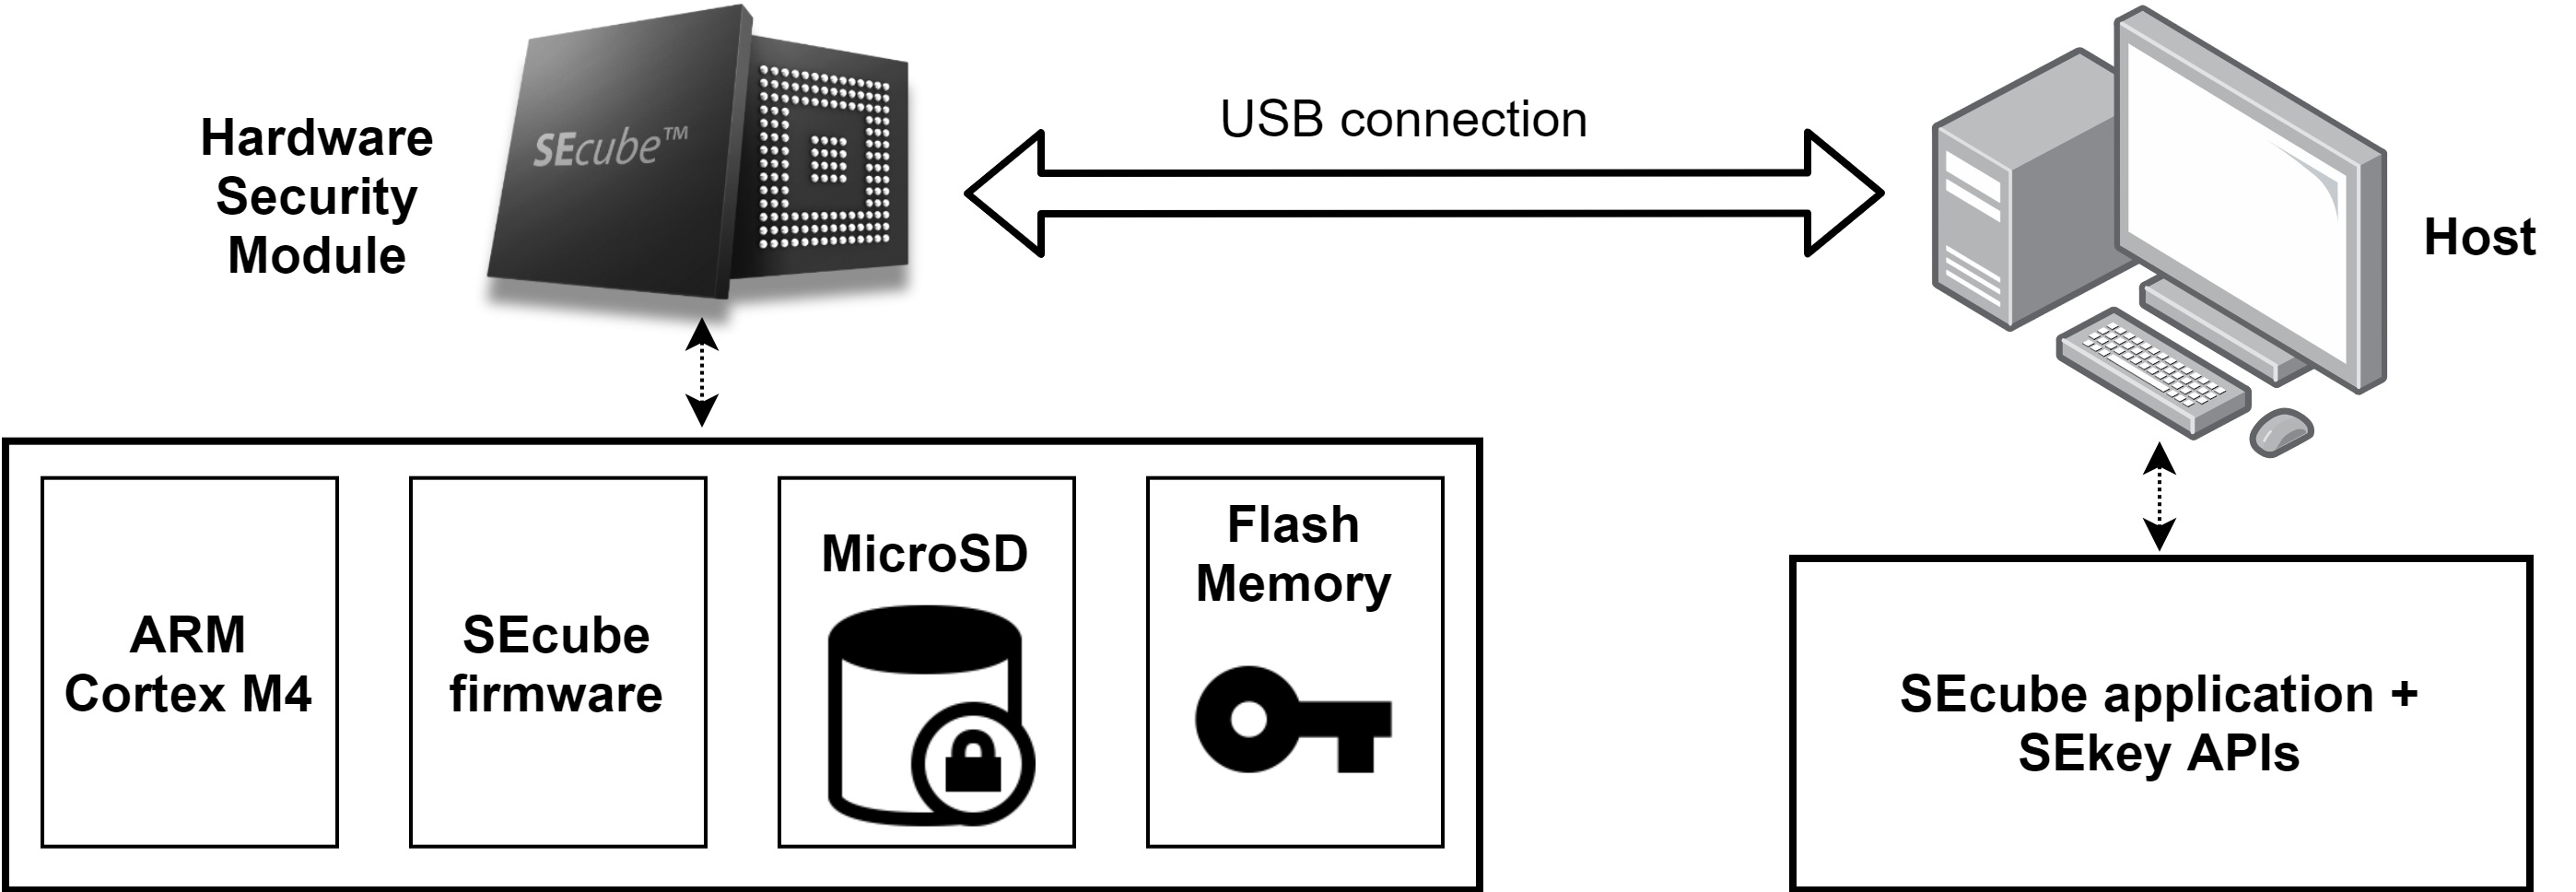
\includegraphics[width=\textwidth]{images/simplearch.jpg}
\caption{This is the image \emph{caption}.}
\label{fig:generalschema} % This is the image label, with which you can refer to the image in any document location.
\end{figure}

This is an image example. Images must ALWAYS be understandable: never introduce images that have text smaller than the text in your document. If you create the images yourself, try not to make them clash too much with the style of your document, and use the same font as this thesis.
If they are not images of your own creation, you MUST reference them. In the caption of the image, you need to insert a citation to the resource from which you took the image, at the end of the caption sentence, before the fullstop.
Each image you enter MUST be referenced in the text, using a formula similar to this:

\begin{center}
Figure \ref{fig:generalschema} describes the architecture of the system.
\end{center}

You can refer to the image using \lstinline{\ref} followed by the image label, that you put in the \lstinline{\label} entry of the figure. Remember to use the word Figure with a capital F. 

Remember that the more your text is adorned with figures, the more understandable, appreciable and readable it becomes.

\section{Section title}\label{examplesection}
This is a section under a chapter. The number of sections also contributes to greater readability of your text, and to a better display of the content in the index. In fact, sections are automatically shown in the Table of Contents. However, try not to make sections shorter than two pages. For smaller portions of your text, use subsections.

You can refer to a section using its label, using the \lstinline{\ref} directive as for images, like this:

\begin{center}
This concept has been explained in Section \ref{examplesection}.
\end{center}

Remember to use the word Section with a capital S. This is also valid for chapters. 

\subsection{Subsection title}
This is a subsection under the section. 

The following is a table.

\begin{table}
\centering
\caption{Preliminary Experimental Results}
\begin{tabular}{| p{3cm} | p{3cm} | p{3cm} |}
    \hline
    \textbf{Benchmark} & \textbf{Inputs} & \textbf{Processing time} \\ \hline
    SHA & Message of 100 KB & 368449 s \\ \hline
    RIJNDAEL & Message of 100 KB & 1083568 s \\ \hline
    DIJKSTRA & Matrix of 100x100 32-bit integers & 324782 s \\ \hline
    STRING & 1331 50-char strings & 178616 s \\ \hline
    BITCOUNT & 12800 32-bit integers & 419545 s \\ \hline
    \hline
\end{tabular}
\label{tab:ar}
\end{table}

If you want to write a formula, you can do like this:

\begin{equation}\label{eq:thiseq}
X_{k}=\sum _{n=0}^{N-1}x_{n}e^{-ik{\frac {2\pi }{N}}n}\quad \quad k=0,\dots ,N-1
\end{equation}

Tables and formulas are extensively documented online, and any doubts about their syntax can be easily resolved with a simple search. As for figures and sections, the same rules also apply to tables and formulas: mandatory reference in the text, possibility to use \lstinline{\label} to label them, and naming with capital letter (e.g., ``as in Table \ref{tab:ar}, as in Formula \ref{eq:thiseq}).

The following is a piece of code:

\begin{lstlisting}
int func(int N, int M) {
  float (*p)[N][M] = malloc(sizeof *p);
  if (!p)
    return -1;
  for (int i = 0; i < N; i++)
    for (int j = 0; j < M; j++)
      (*p)[i][j] = i + j;
  print_array(N, M, p);
  free(p);
  return 1;
}
\end{lstlisting}

You can customize the style of your code, changing the language, the colors of keywords, of comments or the background by changing the settings inside the \lstinline{\lstset} directive found in the main file. Usually, the listings are not referenced within the text as happens for figures, tables, formulas and sections. Do not overdo the code within your text: use it only for short passages (e.g., function prototypes, or 2 to 5 lines of code within a function to help the reader in better understanding the meaning of the text).

You can also write in-text code using the \lstinline{\lstinline} directive, \\
like this: \lstinline{int main(int argc, char** argv);}.


\chapter{Introduction}

The Internet of Things (IoT) refers to the billions of physical devices connected to the internet around the world, all of which collect and share data. For this reason people should consider using more sophisticated security to ensure the data they collect is secure. Nowadays, everyone can control lights from outside the house, control thermostats with their phones,
and order from online stores simply by speaking out loud. One thing that may go unnoticed is that all of this data is very personal and unique to the individual. These details may appear insignificant on their own.
The reality is that these various devices are logging information on shopping habits, location, and even passing conversations and these devices can be vulnerable to all sorts of weaknesses.
The issue arises when people intercept that data, make a copy of it, and then use it for their own purposes.\\
That is where the VPN comes in.\\
A VPN is a Virtual Private Network that encrypts all data sent between a device and a server. Furthermore, it obscures the device's IP address, making it impossible to determine from where the data was sent. For this reason, many companies that allow employees to work remotely will require them to connect to the company's business network via a VPN; sensitive data always takes a secure route to or from the local area network.
If someone decides to use this service to protect their data, it is possible to search a VPN provider, but this solution has a cost, even if it is often reasonable. On the other side, a free implementation will undoubtedly have less support and may be more difficult to use for the average user.\\
Furthermore, it is difficult to implement a VPN on an IoT device because they require a large amount of computational resources. WireGuard as a VPN is becoming increasingly popular because it is simple, employs cutting-edge cryptography, and is also free and open source.

The goal of the project described in this report is to implement a VPN client for FreeRTOS in order to establish a secure communication channel between a client and a server that allows for confidentiality, integrity, and authentication.\\ The choice settled on WireGuard protocol, because of its lightness and simplicity.\\
The ESP32 was chosen as development platform because modules are affordable and provide all of the required functionalities, particularly the WiFi module, the LwIP network stack and the true random number generator. Moreover the company of the ESP32, Espressif, offers a development framework called ESP-IDF which provides a slightly modified version of FreeRTOS.

This paper is divided into several chapters. The second one provides a brief overview of all the topics required to follow the project's development.
The third chapter provides a general overview of project implementation for the ESP32, while the fourth exposes all technical details. The fifth chapter focuses on a similar development, but in a more general scenario, using the FreeRTOS simulator for Linux.
The sixth chapter summarises all of the findings of the research, as well as the issues encountered and potential future projects. The report is concluded in the seventh chapter.
Appendix A contains a detailed user manual for executing, step-by-step, the projects that were developed.
\chapter{Background}
This chapter provides a summary of all of the project's topics. Starting with the main one, what is a VPN and specifically how WireGuard works, followed by an overview of the operating system used, FreeRTOS. There is also a description of the Lightweight IP Stack and of the board used for the project.
\section{VPN}
A VPN is a Virtual Private Network that guarantees confidentiality, integrity and authentication, through a secure communication channel (VPN tunnel).\\
With this service all the Internet traffic is encrypted and the user is able to protect his online identity, in fact it allows to mask the IP (Internet Protocol) and so the real position.\\
The term \emph{Virtual} means that the devices in this network can be located anywhere in the world, and it is not necessary that they are all under the same local network.

\subsection{VPN classification}
There are two types of VPN:
\begin{itemize}
    \item Remote Access VPN: it allows the user to connect to a server on a private network. 
    \item Site-To-Site VPN: it refers to a connection set up between multiple networks which allows secure routing and communication.\\
        Considering the level of reliability and safety, this type of VPN can also be divided in:
        \begin{itemize}
            \item Trusted: Internet Service Provider (ISP) guarantees the data protection.
            \item Secure: it uses encryption protocols to guarantees the creation of a secure tunnel between the private network nodes. In this way the data inside the tunnel are protected against possible external attacks.
            \item Hybrid: it is a mix of a secure VPN and a trusted one.
        \end{itemize}
\end{itemize}

\subsection{How VPN works}
A VPN uses a tunnelling mechanism, that allows the creation of a secure channel between two remote entities.
The data packets sent in this channel are encapsulated by the tunneling protocol and encrypted.\\
In this way the data are protected against possible external attacks and all the traffic is \emph{invisible} in the public network, because the user ip is masked so formally he is not receiving or sending anything.
In the image \ref{fig:vpnTunnel} it can be seen the logical tunnel that protects the data packets.
\begin{figure}[H]
    \vspace{0.5cm}
    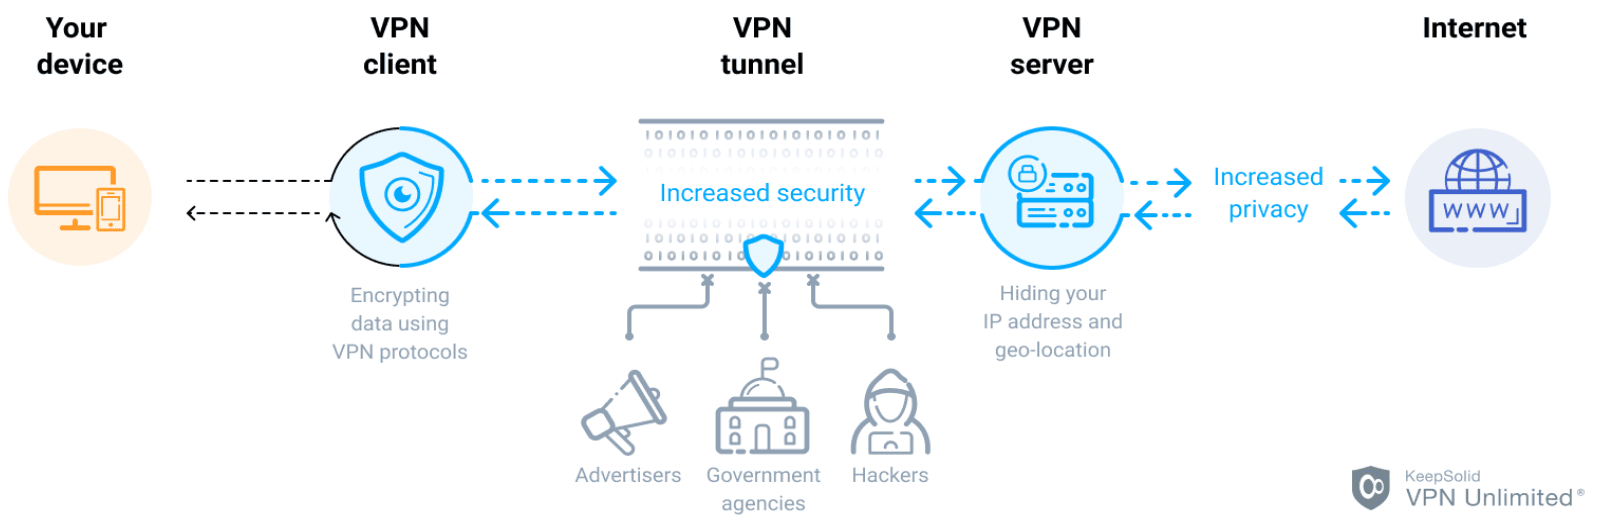
\includegraphics[width=\textwidth, scale=0.25]{images/vpnTunnel.png}
    \caption{VPN tunnelling}
    \label{fig:vpnTunnel} % This is the image label, with which you can refer to the image in any document location.

\end{figure}


\section{WireGuard}
Among all the available VPN, Wireguard \cite{WireGuard} was the one chosen for this project.\\
It is an extremely simple modern VPN which uses state-of-the-art cryptography and it is also Free and Open Source. 
WireGuard is a secure VPN, so through tunnelling, it securely encapsulates IP packets over UDP.\\
How it works is simple: it simply gives a virtual interface which can then be administered using the standard \texttt{ip(8)} and \texttt{ifconfig(8)} utilities. After configuring the interface with a private key and the various public keys of peers with whom it will communicate
securely, the tunnel simply works.

\subsection{How WireGuard works}
The fundamental principle of a secure VPN is an association between peers and the IP addresses each is allowed
to use as source IPs. In WireGuard, peers are identified strictly by their public key, so there is a simple association mapping between public keys and a set of allowed IP addresses.\\
In the following there is an example of a possible crypto key routing table \ref{fig:WGinterface}:

\begin{figure}[H]
    \vspace{0.5cm}
    \includegraphics[width=\textwidth, scale=0.25]{images/wgInterface\_example.png}
    \caption{Cryptokey routing table for a WireGuard Network Interface}
    \label{fig:WGinterface} % This is the image label, with which you can refer to the image in any document location.
\end{figure}

The interface itself has a private key and a UDP port for listening, followed by a list of peers. Each peer is identified by its public key and each has a list of allowed source IPs.\\
It is important that peers are able to send encrypted WireGuard UDP packets to each other at particular Internet endpoints. Each peer in the cryptokey routing table may optionally pre-specify a known external IP address and UDP port of that peer’s endpoint (adding in \ref{fig:WGinterface} an Internet Endpoint in the form IP:UDPport).
It is optional because if it is not specified and WireGuard receives a correctly authenticated packet from a peer, it will use the outer external source IP
address for determining the endpoint.\\
When an outgoing packet is being transmitted on a WireGuard network interface, called wg0, this table is consulted to determine which public key to use for encryption.\\
Using \ref{fig:WGinterface}, when receiving and sending a packet on interface wg0 there will be the following flow:\\
A packet is locally generated and is ready to be transmitted on the outgoing interface wg0:
\begin{enumerate}
    \item The plaintext packet reaches the WireGuard interface, wg0.
    \item The destination IP address of the packet, 192.168.87.21, is inspected, which matches the peer TrMv...WXX0
    \item The symmetric sending encryption key and nonce counter of the secure session associated with peer TrMv...WXX0 are used to encrypt the plaintext packet using ChaCha20Poly1305.
    \item A header containing various fields is prepended to the now encrypted packet.
    \item This header and encrypted packet, together, are sent as a UDP packet to the Internet UDP/IP endpoint associated with peer TrMv...WXX0, resulting in an outer UDP/IP packet containing as its payload a header and encrypted inner-packet. 
\end{enumerate}
A UDP/IP packet reaches UDP port 41414 of the host, which is the listening UDP port of interface wg0:
\begin{enumerate}
    \item A UDP/IP packet containing a particular header and an encrypted payload is received on the correct port.
    \item Using the header WireGuard determines that it is associated with peer TrMv...WXX0’s secure session, checks the validity of the message counter, and attempts to authenticate and decrypt it using the secure session’s receiving symmetric key. If it cannot determine a peer or if authentication fails, the packet is dropped.
    \item Since the packet has authenticated correctly, the source IP of the outer UDP/IP packet is used to update the endpoint for peer TrMv...WXX0.
    \item Once the packet payload is decrypted, the interface has a plaintext packet. If this is not an IP packet, it is dropped. Otherwise, WireGuard checks to see if the source IP address of the plaintext inner-packet routes correspondingly in the crypto key routing table.
    \item If the plaintext packet has not been dropped, it is inserted into the receive queue of the wg0 interface.
\end{enumerate}

\textbf{NOTE}: This explanation part is provided as it reported on the official WireGuard whitepaper \cite{WireGuard}. 

\subsection{Cryptographic Algorithms}\label{sec:WGAlgo}
WireGuard uses state-of-the-art cryptography. Among all the possible algorithms, the ones used in this project are:
\begin{itemize}
    \item BLAKE2S : it is a cryptographic hash function optimized for 8 to 32-bit platforms and it produces digests of any size between 8 bits and 256 bits.
    \item X25519 : it is an elliptic curve DiffieHellman key exchange using Curve25519, which is an elliptic curve offering 128 bits of security (256 bits of key size). It allows two parties to jointly agree on a shared secret using a non-secure channel.
    \item CHACHA20-POLY1305 : it is an Authenticated Encryption with Additional Data (AEAD) algorithm. It combines the ChaCha20 stream cipher (whose input includes a 256-bit key, a 32-bit counter, a 96-bit nonce and plain text) with the Poly1305 message authentication code.
\end{itemize}
\subsubsection{Authenticated Encryption with Additional Data Algorithm (AEAD)}
It is an algorithm that guarantees both confidentiality (through encryption) as well as integrity and authenticity of data.\\
Encryption only provides confidentiality, but the message sent is not protected against modification. So, additional data must be transmitted along with the message to authenticate it. For AEAD this operation takes the form of a MAC (Message Authentication Code).\\
Keyed hash functions are commonly used to generate MACs.


%simone
\section{FreeRTOS}\label{freertos}
FreeRTOS is a real-time OS which is based on a simple kernel, and it is widely used in many embedded systems applications. It is owned and developed by Real Time Engineers Ltd. 
The application could be organized in different threads that could be executed on different type of processors and the execution order is computed by the kernel basing on the priority of the different tasks, which is assigned by the application designer. Usually, the tasks with more strict time requirements have the higher priority with respect to the one more time tolerant. 

\subsection{FreeRTOS distribution}\label{freertosdistribution}
FreeRTOS could be seen as a library composed of many C source files that provides multi-tasking capabilities. Compiling these files with the target application make it able to reach the FreeRTOS API. In order to simplify the development with this library, many different demo projects, that are preconfigured to compile the correct source files, are inserted in the FreeRTOS released folder.\\
FreeRTOS is configured by the FreeRTOSConfig.h header which is used to setup the OS to fit the target application. It contains different configuration in order to set parameters like, for example, the scheduling algorithm. This file must be located in a directory that is part of the application that has been built. 
The official distribution is given with first and second directory as can be seen in figure \ref{fig:freeRTOSFolder} 

\begin{figure}[H]
\vspace{0.4cm}
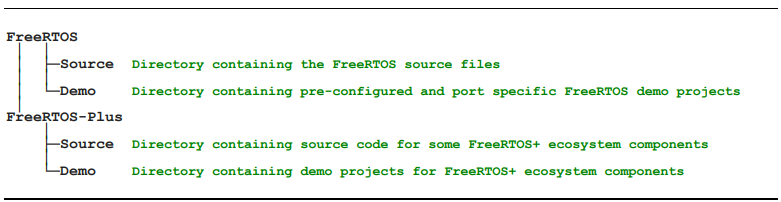
\includegraphics[width=\textwidth]{images/freeRTOS_folder.png}
\caption{FreeRTOS directory tree.}
\label{fig:freeRTOSFolder} % This is the image label, with which you can refer to the image in any document location.
\end{figure}

For more details on FreeRTOS you can check the official site (\cite{FreeRTOSPage}) and the guide (\cite{FreeRTOSGuide})









%Lorenzo
\section{The Lightweight IP Stack - LwIP}\label{lwip}
The Lightweight IP Stack (LwIP) is a very small complete implementation of many network protocols, most importantly it provides everything that is needed for a TCP connection (IP, ICMP, ARP), it is predisposed for some useful protocols like NTP, and PPP.
\\LwIP is built to be easy to port to new platform, which is needed for any hardware change.\\
Only a few files have to be written:
\begin{itemize}
    \item \texttt{cc.h}: definition of basic types (for example u32) for the compiler in use (typically unsigned long or uint32\_t)
    \item \texttt{sys\_arch.c/.h}: functions needed for threaded operation, mainly \texttt{sys\_now()} which returns the current time, and implementations of threads, semaphores and signals that use the underlying resources, usually a Real Time Operating System (RTOS).
    \item \texttt{perf.c/.h}: performance measurement macros (optional).
    \item netif (at least one): a netif is an LwIP network interface. It is described by a \texttt{struct netif}. The netif must implement at least:
    \begin{itemize}
        \item an initialization function, which will be passed to \texttt{netif\_add()} by the application when creating the interface.
        \item some means to call the LwIP input call-back (\texttt{struct netif->input}) when data is received. Usually a thread function started during initialization, or a function to be called periodically by the application. The input call-back is set by \texttt{netif\_add()}, it must be \texttt{tcpip\_input()} for threaded systems, it can be \texttt{ethernet\_input()} or \texttt{ip\_input()} for \texttt{NO\_SYS=1} ports, respectively if LwIP should implement the media access layer (only for ethernet links) or just the network layer (for any other interface).
        \item an output function, to be called by LwIP to transmit data. A pointer should be saved in \texttt{struct netif->output}.
    \end{itemize}
    \item \texttt{lwipopts.h}: LwIP settings, anything that is not defined will take a default value from opt.h.
\end{itemize}
Some example ports are provided in the auxiliary distribution called "contrib" (which indicates code contributed from developers outside the project).

%\subsection{netif: LwIP network interfaces}

LwIP can be ported to a platform that already has a Real Time Operating System, in which case all the facilities for the port already exist in the RTOS, so writing \texttt{sys\_arch.c} is easiest. Care should be taken to ensure that the scheduler is already running when performing operations that use the network hardware, since transmission and reception employ LwIP threads (which are implemented as RTOS tasks). The basic procedure is available at \cite{lwip_port_os}.

LwIP can also be ported to bare-metal platforms that don't have an Operating System. "\texttt{\#define NO\_SYS 1}" \cite{lwip_nosys_doc} must be added to \texttt{lwipopts.h}, and some library functions must be called periodically by user code to poll the network interfaces and other parts of the stack. Threads and other OS features will not be used, so the netconn and socket APIs that need those will not be available to the application. For more information read \cite{lwip_port_nosys}.

There are three APIs available for applications:
\begin{itemize}
    \item Raw / Callback API: \cite{lwip_raw} the user registers call-backs for events (such as reception of one packet). Also used for LwIP internals and for modules, like the WireGuard VPN module, that have to be portable also to NO\_SYS platforms.
    \item netconn API: \cite{lwip_netconn} available only in threaded ports of LwIP. Every feature is accessed through functions named \texttt{netconn\_*()}, some of which block execution while waiting for data or events.
    \item Berkeley / BSD Socket API: \cite{lwip_socket} available only in threaded ports of LwIP. Modeled after the networking APIs of UNIX operating systems, with functions like \texttt{socket()} and \texttt{connect()}. The simple TCP examples written for this project use this API.
\end{itemize}

Given an LwIP port, any application written for LwIP can be linked without modification.










%simone
\section{ESP32}\label{ESP32}
ESP32 is a low-cost, low-power SoC with a Wi-Fi support. It was created by Espressif Systems and there are different versions for different purposes.
Each board of the family could be used for this project.\\
The board that was used in the project (ESP-WROOM-32) has the following specs:

\begin{itemize}
\item Dual-core Xtensa LX6 32 bit (frequency up to 240MHz)
\item 520KB of SRAM
\item 4 MB of Flash memory
\item Wi-Fi 802.11n
\item Bluetooth 4.2
\item Peripherals: SPI, I2C, I2S, UART, CAN 2.0, Ethernet MAC, ADC 12 bit
\item 32 programmable GPIOs
\item Hardware True Random Number Generator
\end{itemize} 

Figure \ref{fig:ESP32FunctionalBlock}. also represents a functional view of a generic ESP32
\begin{figure}[H]
    \centering
    \vspace{0.5cm}
    \includegraphics[ width=0.5\textwidth, scale=0.25]{images/ESP32_functional_block_diagram.png}
    \caption{ESP32 functional block diagram.}
    \label{fig:ESP32FunctionalBlock} % This is the image label, with which you can refer to the image in any document location.
\end{figure}

The TRNG and the WiFi module are fundamental  for the project. The first one is used in the cryptographic algorithms described in section \ref{sec:WGAlgo} to generate a true random source and the latter to create the VPN connection based on lwIP.\\
ESP-IDF can be executed on this board as could be seen in the following subsection
\subsection{ESP-IDF}
ESP-IDF is the development framework used for Espressif SoCs. It contains all the APIs for the ESP32 and scripts to operate the toolchain.\\
This tool provides a version of FreeRTOS, which is based on Vanilla FreeRTOS v10.4.3\\ 
The other software required for development with ESP-IDF are:
\begin{itemize}
\item The toolchain required to compile the code for ESP32
\item Build tools - CMake and Ninja to build a full application 
\end{itemize}
Figure  \ref{fig:espidf} illustrates how the application is built and uploaded on the board.

\begin{figure}[H]
    \centering
    \vspace{0.5cm}
    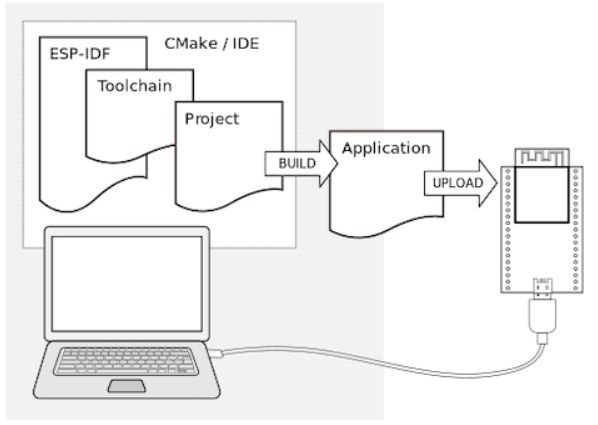
\includegraphics[width=0.5\textwidth]{images/esp-idf.png}
    \caption{ESP-IDF software flow.}
    \label{fig:espidf} % This is the image label, with which you can refer to the image in any document location.
\end{figure}

More details available on the official documentation \cite{ESP-IDF-Page}.



\chapter{Implementation Overview}
This chapter describes, at a high level, how the ESP32 project works, and all of the steps taken during the development phase.

\section{Goal of the project}\label{projectgoal}

The focus of the project is on an implementation of a VPN client on FreeRTOS using an lwIP stack. 
In order to obtain it, some implementation of VPN has been analysed and, among these, as already said in previous chapter, WireGuard was chosen.
Once the VPN is decided, the goal is to port it on a platform that supports FreeRTOS. The possibility considered are three:
\begin{enumerate}
    \item Simulate FreeRTOS on Windows or Linux
    \item Emulate a board behaviour on Qemu
    \item Run FreeRTOS on a physical board
\end{enumerate} 
The starting point was the 3rd option, using the ESP32 board, since it has everything you need.\\
The firmware that has to be obtain therefore must interacts with a WireGuard server and must be able to send and receive data with the latter in a secure way, so guaranteeing confidentiality, integrity and authentication.\\
After having clarified the objectives set, in the next section it's shown how the client VPN is actually implemented.

\section{WireGuard software module}

The software module can be decided in 2 different components:
\begin{enumerate}
\item An internal network interface, that uses the lwIP stack and it is interfaced to receive data on a virtual internal connection, using a private IP, with the internal application
\item Internal cryptographic part, which encrypts and decrypts the data received
\item A peer part, which communicates the encrypted message through the WiFi module of the board on the external network, sending the data to the server
\end{enumerate} 
Therefore, the software module is placed between the application and the external server. This could be observed more in details below.

\section{VPN client-server architecture}
In order to create the VPN connection, the data must be encrypted before reaching the external network, indeed as can be observed in figure \ref{fig:ESP32withVPN}. On the ESP32 board there is an implementation of the WireGuard software module that is able to receive, through a TCP connection, data from an application that want to send a packet to the server.
\\The software module receive the data on his virtual network lwIP interface and encrypts the data using the algorithms described in section \ref{sec:WGAlgo}. Once the data are encrypted, they are sent through the virtual peer of the module (using an UDP connection) to the external network using the WiFi module of the board with a public IP. 
The data sent is encrypted and only the destination WireGuard server can decrypt them, indeed, when the latter receives the packet on his public IP, it is able to decrypt the message and send it to the internal local network with VPN. \\
The same mechanism works similarly if the application receives data from the server, with the WireGuard module that decrypts the data received.

\begin{figure}[H]
    \vspace{0.5cm}
    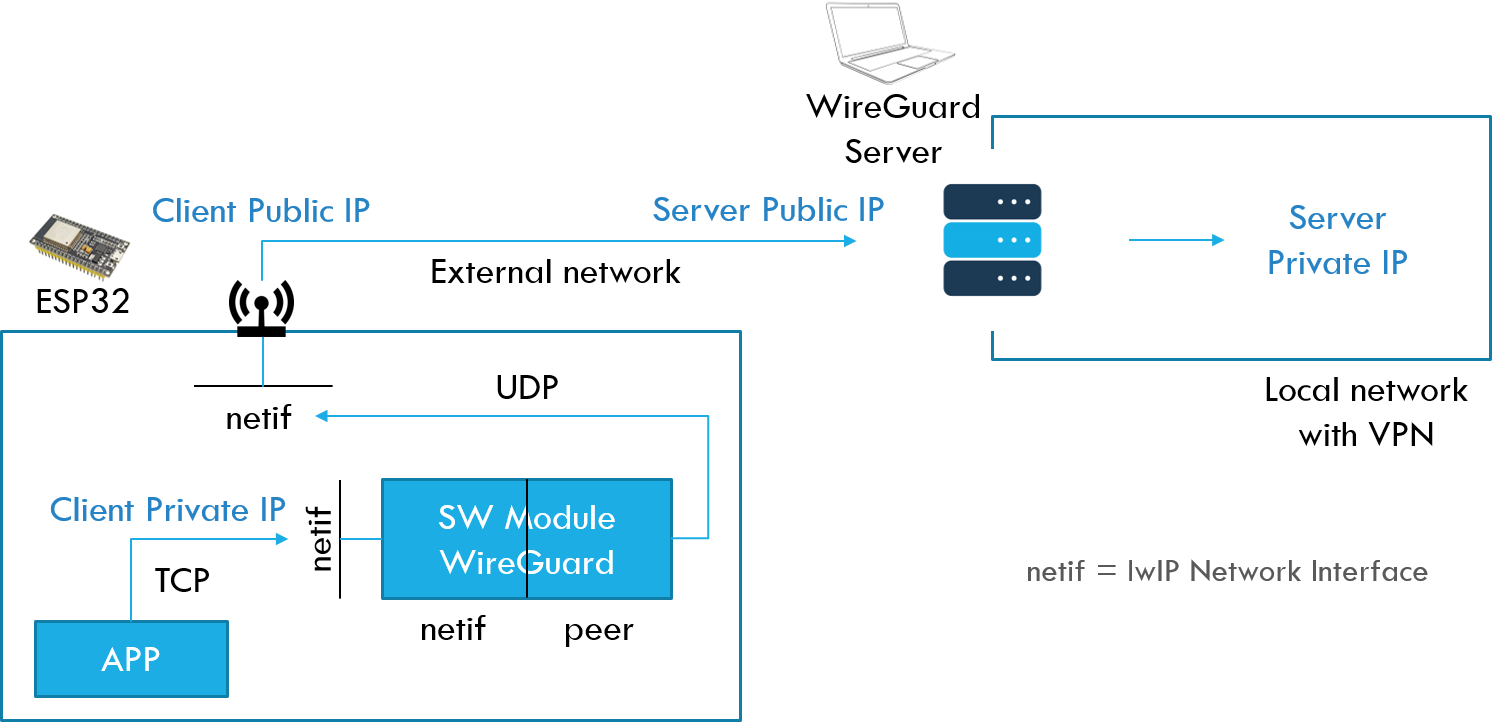
\includegraphics[width=\textwidth]{images/ESP32_whit_VPN.png}
    \caption{Connection between ESP32 and server through VPN.}
    \label{fig:ESP32withVPN} % This is the image label, with which you can refer to the image in any document location.
\end{figure}


\chapter{Implementation Details ESP32}
In this chapter are reported all steps that have been done in order to understand the functionality of ESP-IDF provided by Espressif\cite{ESP-IDF-Page} in order to achieve the goal of the assignment and create the final project presented at the end of the course.
After a general brainstorming, an ESP32 was decided as the chosen board because many useful resources are freely available. Mainly ESP-IDF that is Espressif’s official IoT Development Framework for the ESP32, ESP32-S and ESP32-C series of SoCs. It provides a self-sufficient SDK for any generic 
application development on these platforms, using programming languages such as C and C++.

\section{WireGuard on ESP32}\label{sec:wireguard}

In order to make the ESP32 board able to connect through a VPN tunnel, it is necessary to set up a WireGuard module. This module, as described before, is used to interface the board with the remote server, so related IPs needs to be consistent with the one in the server.\\ 
The WireGuard module \texttt{trombik\_esp\_wireguard} was taken from the Trombik project \cite{wg_trombik} and added in the directory \texttt{Esp32\_tcpprompt\_wg/components}.\\
Then the following line:
\begin{lstlisting}
{REQUIRES trombik\_esp\_wireguard nvs\_flash}   
\end{lstlisting}
was inserted in the file \texttt{CMakeLists.txt} in the directory \texttt{Esp32\_tcpprompt\_wg/main}.\\




\subsection{Related projects}
First of all, it is better to introduce the main projects that was the starting point reference:
\begin{itemize}
    \item Smartalock \cite{wg_smartalock}, which is a C WireGuard implementation for lwIP, which cointains a generic structure (i.e. independent from the platform). 
    As explained in its Readme document the code has four main portions:
    \begin{itemize}
        \item \texttt{wireguard}, which contains the bulk of the WireGuard protocol code and is not specific to any particular IP stack
        \item \texttt{wireguardif}, which contains the lwIP integration code and makes a netif network interface and handles periodic tasks such as keepalive/expiration timers
        \item \texttt{wireguard-platform}, which contains the definition of four functions to be implemented per platform 
        \item \texttt{crypto}, which supports:
        \begin{itemize}
            \item BLAKE2S
            \item X25519
            \item CHACHA20-POLY1305  
        \end{itemize}   
    \end{itemize}
More details on the cryptographic algorithms are discussed in the background chapter (\ref{sec:WGAlgo}).
    \item Trombik \cite{wg_trombik}, is an alpha extension of the previous project, and creates a single WireGuard peer connection using ESP-IDF. This module is also a component of the project that has all the necessary to adapt the Smartalock to an ESP32 board. 
\end{itemize}



\subsection{WireGuard module}
In order to set up the module, the starting point was the ping example present in the Trombik project \cite{wg_trombik}, in order to see if the WireGuard server was reachable. To do that, has been tried the provided example configured with all the parameters like the one on the server.
This example could be divided in:
\begin{itemize}
    \item WireGuard configuration and setup, where all the WireGuard parameters are initialized in \texttt{wireguard\_setup()}, setting:
    \begin{itemize}
        \item private\_key
        \item listen\_port
        \item public\_key
        \item allowed\_ip
        \item allowed\_ip\_mask
        \item endpoint      
        \item port
        \item persistent\_keepalive (i.e. periodically send keepalive packets)
    \end{itemize}
    and then are called:
    \begin{itemize}
        \item \texttt{esp\_wireguard\_init()}, which received the previous variables
        \item \texttt{esp\_wireguard\_connect()}, connects to the corresponding peer 
    \end{itemize}
    \item WiFi and ping, that connects the module to the WiFi and manages the ping communication with server. The WiFi is connected using \texttt{wifi\_init\_sta()} that calls one of the two following functions:
    \begin{itemize}
        \item \texttt{wifi\_init\_tcpip\_adaptor()}
        \item \texttt{wifi\_init\_netif()} 
    \end{itemize}
    the ping instead is managed by \texttt{start\_ping()}, which communicates with the server and respond with a timeout or a success.
    \item time synchronization, necessary to agree during the communication with the server (it is managed by the sync\_time.c)
    \item main, which manages the previous sections in order to run the example and ping the server.
\end{itemize}   
Starting from this configuration, the example provided is used as a reference to build the application.

\subsection{Failed approach}
In a first attempt it was tested also another project from Zmeiresearch \cite{wg_zmeiresearch}, but it was unfeasible to make it work. In a comparison with Trombik it was noticed that maybe it could be due to the absence of a timing synchronization. 

\section{Blinky, Wifi, Component logic}
The first step was to make something run on the ESP32 to understand how the system works. Read the Espressif Documentation for ESP-IDF and for the ESP32 was essential.
Following the guide provided in the Appendix \ref{sec:SysSetupESP32} , a Blinky project was tested. Its directory location is provided here:
\begin{lstlisting}
    esp-idf/examples/get-started/hello_world
\end{lstlisting} 

By doing this the good state of the board was checked.
The next step was to establish an internet connection between the ESP32 and another machine in order to add later the VPN tunnel.
In order to do that a TCP/IP connection was chosen and so implemented starting from the \texttt{Hello\_World} project.
But before that, the WiFi connection needed to be done. The ESP-IDF provides a project where this functionality is provided.
\begin{lstlisting}
    esp-idf/examples/common_components/protocol_examples_common
\end{lstlisting}

In a first attempt the \textit{protocol\_examples\_common} project was included as a component inside the \textit{TCP/IP} project (to understand how to add a component into a project look at the official documentation \cite{ESPcomponents})
\\Then the WireGuard module was analysed starting from two projects described in section \ref{sec:wireguard} in more details. Those two projects were tested standalone and at the end
the Trombik\cite{wg_trombik} project was added as a component in the TCP/IP project. As written in the next section \ref{sec:VPNproject}, in the final version of the project called \texttt{Esp32\_tcpprompt\_wg} the WiFi functions already integrated inside Trombik project were used instead of the WiFi component provided by Espressif. 

\section{TCP/IP communication with WireGuard on ESP32}\label{sec:VPNproject}
After the previous examples, that were propaedeutic to the development of the project, it was possible to implement a TCP/IP communication inside a VPN tunnel.\\ 
The project is located in the directory \texttt{/Esp32\_tcpprompt\_wg}.\\
The task developed for the communication is the following one, and it is located in the file \texttt{main.c}, inside the directory 
\texttt{/Esp32\_tcpprompt\_wg/main}:
\begin{itemize}
    \item \texttt{static void tcp\_client\_task(void *pvParameters)}\\ It contains the main loop of the application, in which there can be found the four main functions:
     \begin{enumerate}
        \item \texttt{socket()} : it creates a TCP socket
        \item \texttt{connect()} : it opens the TCP connection
        \item \texttt{send()} : it sends a message
        \item \texttt{recv()} : it receives a message 
    \end{enumerate}
    In this task it is set which port needs to be used in listening. The one used in this project is 3333.\\
    When the TCP socket is opened, the communication starts and makes possible to have an interaction between the esp32 and the server.\\
    The application that was created was a login-like communication, so the ESP32 asks for some credentials and the user answers.\\
    The ESP32 has a static list of available commands:
    \begin{itemize}
        \item \texttt{Hello from ESP32, please login Username:}\\
        It is the first message sent by the ESP32 which waits for an answers with the user credential. 
        \item \texttt{Password:}\\
        After receiving the username it asks for a password, and waits for the user to answer.
        \item \texttt{Authentication succeeded\\
         Select commands:\\
        - Hello:  to get greetings\\
        - Usage:  to read cpu load\\
        - LogOut: Log Out}\\
        If the combination of username and password are correct, the user can choose one of these commands and will have a different answer.\\
        \item \texttt{Authentication failed, try again...  Username: }\\
        If the username or the password (or both) is wrong, the authentication failed and the esp32 asks again for the credentials.
    \end{itemize}
    
\end{itemize}
After developing this task, the WiFi module and the WireGuard module were taken from Trombik\cite{wg_trombik} and added to our project.\\
When the project is run, the function \texttt{main()} is called and it calls the functions:
\begin{enumerate}
    \item \texttt{wifi\_init\_sta()} : it initializes the WiFi module
    \item \texttt{wireguard\_setup()} : it setups the WireGuard server
    \item \texttt{xTaskCreate()} : it is a FreeRTOS function that receive a task that needs to be created. In this case it receives the \texttt{tcp\_client\_task}
\end{enumerate}
It also checks the time for the timing synchronization, that is necessary for the handshake.
\\An example of the communication can be seen in figure \ref{fig:communicationEx}.
    
\begin{figure}[H]
    \centering
    \vspace{0.35cm}
    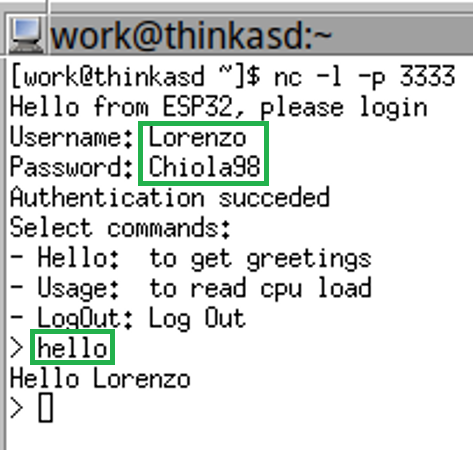
\includegraphics[width=0.4\textwidth]{images/communicationEx.png}
    \caption{Communication output}
    \label{fig:communicationEx} % This is the image label, with which you can refer to the image in any document location.
\end{figure}

It could be seen that the messages sent by the esp32 are the one listed before, and for each of them there is the user answer (the message in the green box).\\


\section{Adding the WireGuard module to iperf and testing performance}\label{sec:iperf_wg}

Between the code examples of ESP-IDF there is an iperf port for the ESP32, available at

\texttt{examples/wifi/iperf/}\\(the actual iperf code is inside a submodule located at \texttt{examples/common\_components/iperf/}).\\
iperf is a common tool used to measure network throughput between two hosts. One will run the tool in server mode, the other in client mode. Random packets of data will be exchanged by the two instances (over TCP by default) to measure the average speed.\\
The iperf port by Espressif is based on another one of their code examples: a command line interface provided over the serial port. Its code is available at

\texttt{examples/system/console/advanced/components/}, which is included as a submodule in iperf. The available commands are iperf itself, \texttt{sta} and \texttt{ap} to configure the WiFi connection (station or access point), and \texttt{free} and \texttt{heap} to measure free ram (in the present or the historical low). A new command can be registered to the console, together with a callback which works much like \texttt{main(int argc, char* argv[])} with arguments passed from the command line.\\
The following procedure shows how to add the WireGuard module from the repository \cite{wg_trombik} to iperf for the ESP32, also adding a command to the text interface.\\
The result should be similar to the contents of the folder \texttt{iperf\_wg/} of the supplied code. It can be useful to compare this folder to the iperf code from ESP-IDF to highlight the differences introduced with the WireGuard module.\\
It is assumed that the provided iperf example was built as a standard ESP32 project without issues.

\begin{enumerate}
    \item Mkdir \texttt{components/} and git clone \cite{wg_trombik} in that folder. The \texttt{components/} folder, if it exists, is automatically searched for submodules by the build system. The only constraint is that a valid \texttt{components/*/CMakeLists.txt} file has to be present for each submodule.
    \item Move the time synchronization code
    
    \texttt{components/esp\_wireguard/examples/demo/main/sync\_time.c / .h} to \texttt{main/}. The rest of the \texttt{examples/demo/} folder can be deleted.
    \item Register a new command to set up the VPN. Take \texttt{main/cmd\_wifi.c / .h} as an example to adhere to the structure of the underlying iperf code. Files \texttt{main/cmd\_wifi.c / .h} were written this way. The new command \texttt{wgup [peer ip address]} starts the VPN tunnel to the other peer. The call-back function is \texttt{wg\_up()}, while the function \texttt{register\_wg()} registers the new command in the command line at start-up.
    \item Integrate the new code in the project:
    \begin{itemize}
        \item As always when adding new source files, it is necessary to add them to the
        
        \texttt{main/CMakeLists.txt} project file so they can be compiled. Add each file name in double quotes after the last C source in the \texttt{idf\_component\_register(SRC "...")} macro.
        \item Include the new header file inside the aggregator header \texttt{cmd\_decl.h}.
        \item Call \texttt{register\_wg()} inside \texttt{app\_main()} to register the new command.
    \end{itemize}
    \item Optionally use the \texttt{menuconfig} system to define options for the WireGuard module. In the supplied code this system is used, so an additional file \texttt{main/Kconfig.projbuild} was created to define some new menu entries which will appear inside the configuration along with the standard options.
\end{enumerate}

It will be now possible to use the command line interface through the serial port monitor.\\
Iperf will work as before, but it will be possible to send the \texttt{wgup} command to set up the VPN tunnel, so that any further traffic originating from the inside of the esp32 will be routed through the tunnel.\\
\ref{fig:iperf_wg_long} is a screenshot of the serial monitor session after running iperf, starting the VPN, and running iperf again this time inside the VPN tunnel. Note that the IP address changes for the second run; also the IP address of the first iperf server is the same as the IP address of the WireGuard peer, since they were running on the same computer.
This run was used to record performance and RAM usage, see \ref{sec:performance}.

\begin{figure}[H]
    \centering
    \vspace{0.5cm}
    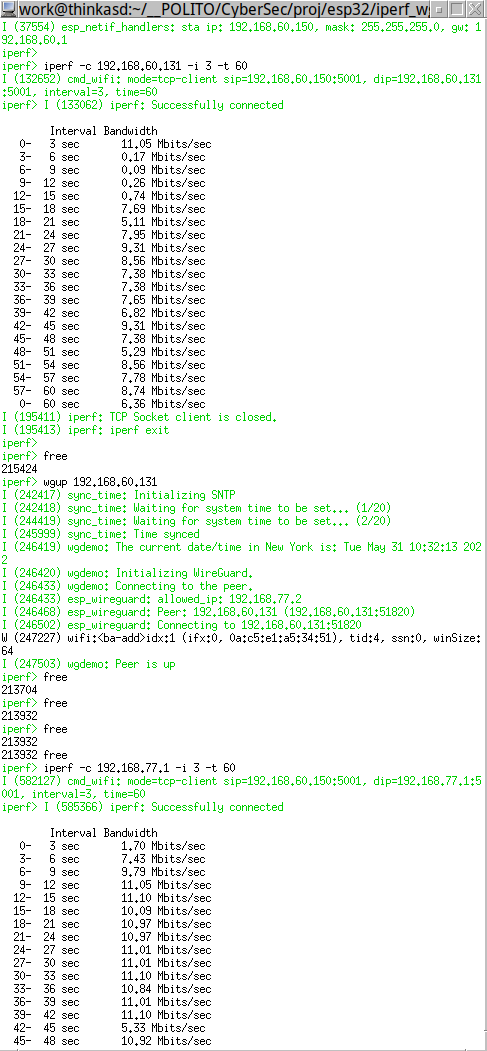
\includegraphics[ width=0.4\textwidth]{images/iperf_wg_serial_monitor_long.png}
    \caption{iperf running on the ESP32 both outside and inside the VPN tunnel. The remote computer is reachable both from inside and outside the VPN, it is running iperf in server mode: \texttt{iperf -s}}
    \label{fig:iperf_wg_long} % This is the image label, with which you can refer to the image in any document location.
\end{figure}



\chapter{Running the VPN in the FreeRTOS simulator for Linux}
FreeRTOS already has a port that runs as a native process in Posix systems, known as the Posix simulator. LwIP also has support for running under Linux using virtual network interfaces. In this chapter LwIP is configured to run in FreeRTOS (which is a very common use case with a port already existing) while using a Linux virtual network interface. Finally, the WireGuard module is added.

\section{Build FreeRTOS for Linux (simulator)}
FreeRTOS supports running as a process inside a Posix system for simulation purposes.\\
The Posix port implements tasks as pthreads, however only one thread will be running at any time, dictated by the FreeRTOS queue.\\
Each thread receives Posix signals to simulate interrupts (mainly SIGALARM for the System Tick interrupt), so that execution is periodically passed back to the task queue, which then restarts one of the threads with SIGUSR1.
See also \href{https://www.freertos.org/FreeRTOS-simulator-for-Linux.html}{(simulator doc)}, or the comments in the port files in \texttt{FreeRTOS/Source/portable/ThirdParty/GCC/Posix/} of the FreeRTOS distribution.
A simulation port of FreeRTOS for Windows is also available. It was not tested for this project because the limited available networking options meant adding LwIP would have been impractical.
\\Note that FreeRTOS loses any real time guarantee when ported to Posix, since the latter is not deterministic.
Scheduling still follows the same criteria that would apply on an embedded system, and operation with a 1 ms system tick is possible on an unloaded laptop CPU. Problems might arise inside virtual machines or on old hardware. Missing some system ticks would not be critical for this project.


\section{Adding LwIP on top of FreeRTOS}
LwIP will not be running on an embedded system, but rather in a simulated environment. The compiler will be a standard gcc for Linux, while the underlying operating system will be FreeRTOS. A Unix TAP virtual network interface will be created to allow LwIP to connect to something outside the FreeRTOS simulator.
\\This procedure shows how to make LwIP available to FreeRTOS applications such as the blinky example (see \ref{sub:linux_blink} for details and build instructions).
The expected result of these steps should be similar to the contents of the folder \texttt{Posix\_GCC\_lwip1/} of the supplied code, which was derived from blinky. In that code A TCP connection is established to another device on the network; the same messages that are displayed on \texttt{stdout} by blinky are sent over TCP too.

\subsection{tapif: the network interface}\label{TapInfo}
A Unix TAP is a virtual network interface that behaves mostly like an Ethernet interface. On the OS end it behaves like any other network interface of the system, it can be configured with the \texttt{ip link / ip addr / ip route} utilities and can have IP addresses. The other end of the TAP is not a driver for a physical interface, rather it can be controlled through the \texttt{open() / close() / read() / write()} system calls by a user application that wishes to emulate a NIC.\\
TAPs are commonly used by VPN user space clients (not WireGuard) to provide a network interface that appears connected to the VPN local network, and by virtual machines to give network access to guest systems.
\\To set up a TAP in Linux operating systems see Section \ref{sec:WGRtos}.

\subsection{LwIP setup}
\begin{enumerate}
    \item Download the two LwIP packages: both
    \begin{itemize}
        \item the sources of LwIP itself \cite{lwip_download}, and
        \item the contributed code \cite{lwip_contrib_download}, which contains some ports that are going to be used.
    \end{itemize}
    \item Write the \texttt{lwipopts.h} file:
    \begin{itemize}
        \item thread defines: these should already be defined when starting from a \texttt{lwipopts.h} file with \texttt{NO\_SYS==0}. For a ready-made example see \texttt{Posix\_GCC\_lwip1/lwip/lwipopts.h}. Determining the values needed without knowing the internals of LwIP essentially requires to study the internals, either from the (excellent) documentation or by debugging the program hunting the reasons for trace dumps, which are rarely obvious. If at all possible, start from an \texttt{lwipopts.h} from a similar application.\\
        All available parameters can be read from the defaults file \texttt{lwip/src/include/lwip/opt.h}.
        \item Please also add the following lines to \texttt{lwipopts.h}:\\
        \texttt{\#define MEMP\_NUM\_SYS\_TIMEOUT    6   // because the default is not correct (see\\opt.h line 508)}\\
        \texttt{\#define PBUF\_POOL\_BUFSIZE        256 // if you wish to use the WireGuard module,\\because of an assumption done in that code, see} \ref{sec:addwglinuxsection}
    \end{itemize}
    \item Add the sources of LwIP to the project
    \begin{itemize}
        \item mkdir \texttt{lwip}
        \item copy the \texttt{src/} directory from the LwIP distribution to \texttt{lwip/}
    \end{itemize}
    \item Copy the port files
    \begin{itemize}
        \item mkdir \texttt{lwip/port/}
        \item copy the contents of \texttt{ports/freertos} from the LwIP contrib distribution to \texttt{lwip/port/}. These are the \texttt{sys\_arch.c/h} files that implement threads, semaphores, mailboxes and mutexes based on FreeRTOS.
        \item copy \texttt{ports/unix/port/include/arch/cc.h} from the LwIP contrib distribution to\\\texttt{lwip/port/include/}. This header contains the basic definitions for compatibilitiy with the Linux-native \texttt{gcc} compiler.
        \item copy \texttt{ports/unix/port/netif/} from the LwIP contrib to \texttt{lwip/port/}. Only \texttt{tapif.c} and \texttt{include/tapif.h} are really necessary.
        \item remove error handling: comment the call to \texttt{perror()} at \texttt{line 427 in tapif.c}.\\
        This netif was built for LwIP over straight Linux, but we are running LwIP over FreeRTOS inside Linux. The system tick in the FreeRTOS port for Linux is implemented using a Posix Signal that is generated every millisecond to interrupt the running task and run the scheduler. When the signal is delivered it interrupts any blocking system call, in particular the system call used by tapif to communicate with the Unix TAP returns \texttt{EINTR}. The call can be restarted without special considerations, so the error can be safely ignored.
    \end{itemize}
    \item Add the necessary LwIP files to the variables \texttt{SOURCE\_FILES} and \texttt{INCLUDE\_DIRS} in the \texttt{Makefile}. The list was determined by trial and error, building the project and resolving symbols that were missing while linking, and by referencing some examples. Note the use of wildcards in the \texttt{Makefile}:
    \begin{itemize}
        \item \texttt{lwip/src/core/*.c}, \texttt{lwip/src/core/ipv4/*.c}: basic LwIP functionality.
        \item \texttt{lwip/src/api/*.c}: this project uses the BSD socket API, which is the most abstract, so all the files here are needed. A project which only uses the \texttt{RAW} or \texttt{netconn} APIs could shed some size by not building the socket API.
        \item \texttt{lwip/port/sys\_arch.c}: the FreeRTOS port layer.
        \item \texttt{lwip/src/netif/ethernet.c} which is almost always used by ethernet-based netifs, and \texttt{lwip/port/netif/tapif.c} which is the outside-facing netif we are going to use.
        \item Include directories: \texttt{lwip/src/include} for LwIP and \texttt{lwip/port/include} for the port layer (here are \texttt{sys\_arch.h}, \texttt{cc.h} and optionally \texttt{perf.h}). Also include whatever directory contains \texttt{lwipopts.h} (it can be found in folder \texttt{lwip/} in the supplied code, but it could be saved in \texttt{lwip/port/include} for simplicity).
    \end{itemize}
    \item Write some basic application code. A finished example derived from the \texttt{Posix\_GCC} FreeRTOS example is given in the \texttt{Posix\_GCC\_lwip1/} folder of the supplied code.\\
    This example does the following:
    \begin{itemize}
        \item in \texttt{main\_blinky()}:
        \begin{enumerate}
            \item initialize LwIP with \texttt{tcpip\_init(NULL, NULL);}
            \item create the outside-facing network interface of the tapif type with \texttt{netif\_add()}
            \item create a TCP socket (internally to LwIP) with \texttt{socket()}
        \end{enumerate}
    
        \item in a separate task function called \texttt{prvTCPConnectorTask}(), run after starting the scheduler:
        \begin{enumerate}
            \item establish the TCP connection with an external host on port 3333 with \texttt{connect()}
			\item in general, run any operation that communicates through a netif \textit{only after starting the scheduler}, or else the netif will not be functional, making the operation hang or fail.
        \end{enumerate}
    \end{itemize}
    Use Netcat to listen on TCP port 3333 on the computer which runs the simulator. Use the command \texttt{nc -v -l -p 3333}.
\end{enumerate}

\section{Adding the WireGuard module to an LwIP project}\label{sec:addwglinuxsection}
This section will guide the reader through the process of adding the WireGuard module to the basic FreeRTOS + LwIP setup obtained in the previous section.\\
The end result of this procedure should be similar to the contents of the folder \texttt{Posix\_GCC\_lwip2\_wg/} of the supplied code.
\begin{enumerate}
    \item Download the wireguard-lwip module either from \cite{wg_smartalock} (original, preferred), \cite{wg_trombik} (ESP32 port, identical clone of (1)), and copy it to a folder in the project (see \texttt{wireguard-lwip} in the supplied project).
    \item Ensure that \texttt{PBUF\_POOL\_BUFSIZE} is defined to be more than 134 in \texttt{lwipopts.h}. This is needed because the WireGuard module expects to get the handshake response (92 bytes), received from the remote peer, inside a single pbuf. The pbuf pool contains space for a number of pbufs, the data buffers of LwIP. When a packet is too big for one pbuf, a singly linked list of pbufs is created to hold the whole message. This quantity of data also has 42 bytes of overhead for Ethernet, IP and UDP, totalling to 134 bytes.
    \item Create a platform support file (\texttt{wireguard-lwip/src/wireguard-platform\_unix\_freertos.c} in the project code). Implement in this file four functions needed by the WireGuard module. Note that you can just use the example \texttt{wireguard-lwip/src/example/wireguard\_platform.c} as a basic, workable but insecure version.
    The four functions are:
    \begin{itemize}
        \item \texttt{wireguard\_random\_bytes()} should be a strong random number generator. Note that \textbf{the default example is a weak pseudo random number generator, unsuitable for real-world usage}. On a Linux platform it could be implemented to read /dev/random, however this involves system calls which are easily broken by the FreeRTOS simulator, as was shown for the tapif interface in the last chapter. In this case the \texttt{read()} call could be interrupted, making the function return uninitialized values or some predefined value, like zero, which would critically weaken the cryptographic system anyway, unless a more complete solution is developed.
        \item \texttt{wireguard\_sys\_now()} just returns LwIP's \texttt{sys\_now()} which is a 32 bit unsigned number of milliseconds elapsed from an epoch (in this port the epoch is the start of simulation). Note that this time will wrap around after less than 50 days.
        \item \texttt{wireguard\_tai64n\_now()} returns the tai64n timestamp (specification: \cite{tai64_timestamp}) used in the WireGuard packets. It is essential that this timer increases for every new packet, otherwise the remote peer will just drop the packets.\\
        The example platform file implements this function using \texttt{sys\_now()}, which would break the connection after 49 days, until the server is killed and restarted.\\
        \texttt{wireguard\_tai64n\_now()} was edited to make it return the current time of the underlying Linux OS. The solution uses the \texttt{time()} C library function which, in principle, could generate system calls. However, most of the time no system calls are made, and the function is only used on handshakes, which happen every two minutes by default. For these reasons the probability of an error breaking a \texttt{time()} call is low, and the solution was demonstrated to work well in practice. Using the correct time also avoids the annoyance of restarting the server every time the simulation is killed and restarted, since the timestamp keeps increasing instead of resetting to 01/01/1970.\\
        \item \texttt{wireguard\_is\_under\_load()} just returns false. This could be made to return true if the system is experiencing load above some threshold. When true, the WireGuard module will send out cookies instead of handshake responses, and only accept handshakes having a non-zero mac2 field, which needs the cookie to be computed (see the DoS mitigation section of the protocol description \cite{wg_protocol_dosprevent}). This mechanism would provide limited protection against overload and DoS attacks, since handshaking is relatively expensive compared to ordinary communication.
    \end{itemize}
    \item Initialize the tunnel in the application code, the same way as it is done for the ESP32 platform (see \texttt{wireguard-lwip/src/esp-wireguard.c} from the repository (2) which was also used for the ESP32.).\\
    The code cannot be copied exactly from the ESP32 port however, because it uses many functions from \texttt{esp-idf}.\\
    The same operations were adapted into the task \texttt{prvTCPConnectorTask()} and the function \texttt{unix\_wireguard\_setup()}.
    The operations performed are:
    \begin{itemize}
        \item netif\_add() to create an internal netif of the type used by \texttt{wireguard-lwip}. This will be the VPN termination inside the the target device (simulator in this case).
        \item \texttt{wireguardif\_add\_peer()} to configure the connection to the remote peer
        \item \texttt{wireguardif\_connect()} to initiate a handshake with the remote peer. This phase can be delayed until the connection is actually needed, as is the standard behavior on the Linux and Windows implementations.
        \item wait for the tunnel to be open by calling \texttt{wireguardif\_peer\_is\_up()}
    \end{itemize}
    It may be useful to also resolve the IP address of the remote peer as in 
    
    \texttt{wireguard-lwip/src/esp-wireguard.c}. 
    
\end{enumerate}

\section{Failed approach}
The initial goal of the project was to have a working VPN inside FreeRTOS, so the first networking stack to be considered was FreeRTOS's own FreeRTOS+TCP (the name is somewhat misleading, since it is a complete networking stack). It was not possible for the team to compile a usable demo for Windows or Linux. In particular the virtual network interface based on PCAP was thought to be the culprit.\\
PCAP is the library used by WireShark \cite{WireShark} to capture traffic from a network interface on many operating systems. It is used to provide access to the network in the FreeRTOS+TCP Linux and Windows simulators, by reading and injecting packets from and to a physical Ethernet interface of the host system.\\
A PCAP netif also exists for LwIP on Linux (\texttt{ports/unix/port/netif/pcapif.c} in the contrib package), but it was discarded in favour of the tapif because of the experiences with PCAP in FreeRTOS+TCP.
It was also not clear if PCAP could attach to a virtual TAP interface for experimenting inside a single computer or virtual machine, while the tapif is built for that.



\chapter{Results}
This chapter demonstrates that the communication between the Client and Server is encrypted as expected, as well as the obtained performance on the ESP32 board.
All issues identified during the project's development are reported and explained. A small section with possible future works is also described.    

\section{Encrypted communication checking}
After developing the project application, the packets sent during the communication where analysed through WireShark \cite{WireShark}, which is a free and open source packets analyser.
In this way it was possible to test that the interaction between the ESP32 and the user was really under a VPN protocol, and so correctly encrypted.\\
Below there are two WireShark capture: in these the packet that was captured was the one containing the user password, because it is the most vulnerable data exchanged.

\begin{itemize}
    \item In Figure \ref{fig:WSpublic} there is the capture of the packet in the public network.\\It could be seen that the source and destination IPs are the one of the physical devices, and the communication is happening under a WireGuard protocol.\\Moreover the content of the packets is not visible, and so it has been successfuly encrypted.
    \item In Figure \ref{fig:WSwg} there is the capture of the packet in the WireGuard Network Interface.\\In this case the source and destination IPs are the one assigned by WireGuard Interface, and it could be seen that the packet sent is exactly the user password, so the packet exchange during the communication is the correct one.\\
\end{itemize}

\begin{figure}[H]
    \centering
    \vspace{0.5cm}
    \includegraphics[width=\textwidth, scale=0.25]{images/WS\_publicNet.png}
    \caption{WireShark capture public Network}
    \label{fig:WSpublic} % This is the image label, with which you can refer to the image in any document location.
\end{figure}

\begin{figure}[H]
    \centering
    \vspace{0.5cm}
    \includegraphics[width=\textwidth, scale=0.25]{images/WS\_wgNet.png}
    \caption{WireShark capture WireGuard Network Interface}
    \label{fig:WSwg} % This is the image label, with which you can refer to the image in any document location.
\end{figure}

\section{Performance and resource consumption}\label{sec:performance}
No performance measurements were made on the FreeRTOS simulator for Linux, since it is very different from an actual embedded device.
Program sizes are also influenced by C library code needed to interface with the host, since the whole simulation is compiled into a single executable file.
\\Performance was evaluated on the ESP32 platform using the \texttt{iperf} port provided in the \texttt{ESP-IDF} SDK with the \texttt{wireguard-lwip} module added, see chapter \ref{sec:iperf_wg}.
\\The WiFi network was too slow in the experiments conducted to determine if the cryptography was CPU bound. The best throughput achieved was 11 Mbit/s both directions, both inside and outside the WireGuard tunnel.\\
While this result is not conclusive, it clears the envelope for many applications with limited bandwidth requirements.
Also, many real-world scenarios replicate the same conditions yielding the same or much worse link speeds.
All in all, the communication will not be CPU-bound in most practical cases.
\\Resource consumption was low enough for the ESP32, although this should be evaluated for each platform.\\
37 kilobytes of ROM are needed for the WireGuard module, including the very basic configuration command described in the dedicated chapter. This was deduced from binary sizes at compile time: \texttt{idf.py build} reports a number of used bytes in hexadecimal after the build is complete.\\
For an ESP32 this should be an acceptable quantity of flash for most projects, especially considering the operating system requires 600 kB of flash.
\begin{figure}[H]
    \centering
    \vspace{0.5cm}
    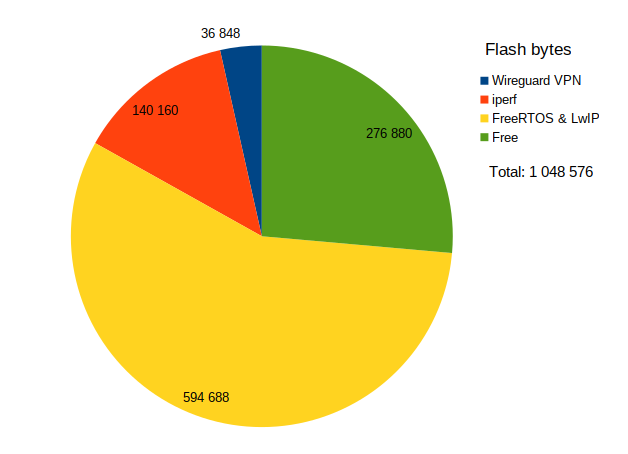
\includegraphics[width=0.5\textwidth, scale=0.25]{images/iperf_flash_footprint.png}
    \caption{iperf with WireGuard: flash memory footprint contributions}
    \label{fig:iperf_flash_piechart} % This is the image label, with which you can refer to the image in any document location.
\end{figure}

RAM heap usage on the ESP32 was 1700 bytes at idle and 7 kilobytes while running iperf. This was reported using the \texttt{free} and \texttt{heap} commands available in the serial console of the iperf port, see \ref{sec:iperf_wg} and \ref{fig:iperf_wg_long}.\\
The ESP32 has 500 kB of internal RAM, of which 220 kB are usable by applications.

\section{Known Issues}\label{sec:problems}
This report shows how to set up a basic VPN tunnel using WireGuard on different cases, however some issues were left unfixed.
\begin{itemize}
    \item Every procedure described works as intended on Linux systems only. On Windows platforms WSL is available, however it does not provide a complete Linux system, and a common virtual machine could be more useful. Most notably:
    \begin{itemize}
        \item WSL 2 is basically a virtual machine, so networking is more complicated (a virtual interface connects to the internet through NAT, \textbf{hyper-v virtual ethernet adapter} issues) and no server can easily run from inside the VM. Also connecting serial devices (which is needed to flash a firmware onto ESP32 chips) requires setting up USB pass-through every time the device is plugged in, which sums up to one command in the Windows host and one command inside WSL.
        \item WSL 1 offers better compatibility. There were no problems with networking, but USB devices problem still remain. It is hard to fix and even so, the build process was really slow (10-15 min on a performant machine). 
        \item Oracle VirtualBox was most practical, offering one-click USB pass-through configuration, and bridged networking that was functional over WiFi too.
    \end{itemize}
    Networking was especially important, because some tools (most notably Netcat) are missing in Windows.
    
    \item 32 bit \texttt{sys\_now()} timestamp: on most LwIP platforms the TAI64N timestamp necessary for WireGuard is obtained from the \texttt{sys\_now()} function of LwIP that returns a 32 bit unsigned millisecond count that overflows every 49 days. The timestamp is always between 01/01/1970 and 18/02/1970. While it is not a problem that the date is far in the past, when the timestamp overflows, or when the device reboots, the date and time go back to a previous instant (01/01/1970). The WireGuard server will reject all handshake packets with an earlier timestamp than the last received, so communication will not be possible until the server is killed and restarted.
    
    \item The random number generator used in the Linux simulator port is not cryptographically secure. 
    See the \texttt{rand()} call inside \texttt{wireguard\_random\_bytes()} in file 
    \begin{lstlisting}
    wireguard-lwip/src/wireguard-platform_unix_freertos.c
    \end{lstlisting}
    Although security was not needed for the simulation, it should be clear that this flaw compromises the whole cryptosystem. A strong random number generator should be implemented for any practical application, as was done for the port to the ESP32 platform.
    
    \item A large number of TCP retransmissions is sometimes generated by the peer using the \textbf{wireguard-lwip} module, usually for an interval of up to 10 seconds, even in perfect conditions (like TAP networking). While performance is very good, this issue should probably be addressed before a practical application is deployed, as there is the potential for some important flaw to be the cause of such a seemingly random malfunction.
    \item All the test on the esp32 have been done using the ESP-IDF version 4.4.1. The latest version available at the time of writing this paper (v5.0.0) does not work with the presented project.
\end{itemize}

\section{Future Works}

The following two important steps are still missing to produce a usable solution:
\begin{itemize}
    \item User friendly configuration of the VPN keys and static IPs. This can be added along the configuration of the WiFi access parameters, keeping in mind that it may not be practical to type two 44-character long keys on a small keyboard or on a number-only keyboard.
    \item Internet routing was not tested nor desired for this project, communication with a single computer was enough. While potentially no changes to the \texttt{wireguard-lwip} module may be needed, the configuration becomes more involved on any peer that has to route traffic to other hosts inside the VPN, be it on a physical local network or to other connected WireGuard peers.
\end{itemize}



\chapter{Conclusions}
Starting with the ESP32 board and then porting in simulation on Linux FreeRTOS, the goal of implementing a VPN Client for FreeRTOS was met.
Several issues arose during the project's development. The first step was to research what a Virtual Private Network is, as well as its functions and how to use it.
\\Following some evaluations, WireGuard was selected as the protocol to create an encrypted communication that ensures confidentiality, integrity, and authentication.
The ESP32 was chosen as the client's development board because it provides all of the required utilities at a low cost.
The Espressif's official IoT Development Framework (ESP-IDF) functionalities were studied in order to use them on the board.
\\While browsing the internet, examples of previously created WireGuard implementations on IoT devices were discovered and used as a starting point for the project.
To simulate a simple packet transmission, a TCP/IP port on a Linux machine was opened, and the ESP32 was used as the sender.
Following the successful communication, the WireGuard module was added to ensure a secure channel.
To ensure that the packets were encrypted, an Internet traffic analyser was used.
So, after the previously described implementation, it was easier to understand how the WireGuard module works and how to configure it. This enabled it to be ported in a more general scenario using the FreeRTOS simulator for Linux.
\\All of the work done allowed the establishment of a raw TCP/IP communication, but a more complex application exploiting the full potential of a VPN could be developed.
Other improvements must be made before this solution can be used in a real-world scenario.

%\begin{thebibliography}{9}
% The bibligraphy is mandatory. Here you have a couple of examples (remember to put references in the text).
\bibitem{texbook}
Donald E. Knuth (1986) \emph{The \TeX{} Book}, Addison-Wesley Professional.

\bibitem{lamport94}
Leslie Lamport (1994) \emph{\LaTeX: a document preparation system}, Addison
Wesley, Massachusetts, 2nd ed.
    
\end{thebibliography}

%%%%%%%%%%%%%%%%%%%%%%%%%%%%%%%%%%%%%%%%%%%%%%%%%%%%%
    
% HERE IS WHERE YOU INCLUDE YOUR APPENDICES (IF ANY)

\appendix
\chapter{User Manual}
\label{usermanual}

\section{ESP32 System Setup}\label{sec:SysSetupESP32}
In this Section, the set of both hardware and software resources required to set up the ESP32 are outlined. 
At the end of this Section, you will have acquired a clear overview of the
prerequisites to set up the environment and run a project. It is strongly recommended to use a virtual machine (use Virtual Box\cite{virtualbox}) 
or machine with a Linux distribution (i.e. Ubuntu Linux\cite{Ubuntu}) installed as operating system and to follow this guide to set up everything.

\subsection{Hardware resources}

\begin{itemize}
  \item \textbf{ESP32 board}.
  \item \textbf{USB cable} - USB A /micro USB B
  \item \textbf{Computer} running Windows, Linux, or macOS
\end{itemize}

This document will focus only on the implementation for the Linux environment. In case of using a virtual machine, 
make sure that the USB ports are visible to your system and internet connection is provided by WiFi bridge (take a look in Known Issues \ref{sec:problems}).

\subsection{Software resources}
You need the following tools:

\begin{itemize}
  \item \textbf{Toolchain} to compile code for ESP32
  \item \textbf{Build tools} - Cmake and Ninja to build a full Application for ESP32
  \item \textbf{ESP-IDF} that essentially contains API (software libraries and source code) for ESP32 and scripts to operate the Toolchain
  \item \textbf{IDE} for C language, on your choice, to edit better the code (OPTIONAL, not covered in this report) 
\end{itemize}

\section{Guide for Linux}
This section provides a summary on getting everything installed and ready to use on Linux (Ubuntu or Debian).
All the reported material is based on the official guide provided by Espressif\cite{Espressif} end various trials.\\
\\\textbf{NOTE}: Install process of Oracle VirtualBox VM and a Linux distribution on it, is not reported in this paper. 

\subsection{Step 1 - Install Prerequisites}
In order to use ESP-IDF with the ESP32, some software packages need to be installed.
Open a terminal and run the following command:

\begin{lstlisting}
sudo apt-get install git wget flex bison gperf python3 python3-venv pip
cmake ninja-build ccache libffi-dev libssl-dev dfu-util libusb-1.0-0
\end{lstlisting}

\subsection{Step 2 - Get ESP-IDF}
To build applications for the ESP32, software libraries provided by Espressif are needed.
\\Download it from here \cite*[\href{https://github.com/espressif/esp-idf.git}{ESP-IDF}]{Git_ESP}
\\Or open a Terminal, and run the following commands:

\begin{lstlisting}
mkdir -p ~/esp
cd ~/esp
git clone -b v4.4.1 --recursive 
    https://github.com/espressif/esp-idf.git esp-idf-v4.4.1
\end{lstlisting}

\textbf{NOTE}: Is strongly recommended to use the ESP-IDF v4.4.1
\subsection{Step 3 - Set up the tools}
Aside from the ESP-IDF, you also need to install the tools used by ESP-IDF, such as the compiler, debugger, Python packages, etc, for projects supporting ESP32.

\begin{lstlisting}
cd ~/esp/esp-idf-v4.4.1
./install.sh ESP32
\end{lstlisting}

\subsection{Step 4 - Set up the environment variables}\label{sec:envSetup}
This step \textbf{must} be executed every time a new Terminal is opened in order to build, flash, etc.
\\In the terminal where ESP-IDF is going to be used, run:

\begin{lstlisting}
. $HOME/esp/esp-idf-v4.4.1/export.sh
\end{lstlisting}

\section{Start the TCP/IP WG project on ESP32}\label{sec:WGprog}
This project is located in the \textbf{ESP32\_tcpprompt\_wg} directory.

Before continue in this section is recommended to set up the Wireguard server, a small guide is provided in section \ref{sec:server} of the Appendix. 
Is strongly recommended to use a Linux Machine or an Android device as a Server. 
Remember to generate the Keys, see in section \ref{sec:server}
This is because for the simple TCP/IP communication built for this project, Netcat is needed to listen on a specific port and it is only available for Linux and Android.
Here are reported the Crypto key Routing Tables WireGuard network interface on both client and server side.

\textbf{Server}:
\begin{lstlisting}
[Interface]
Address = 192.168.77.1/24  # Network Interface IP addr. of the Server
ListenPort = 51820  # default Listening port for UDP communication
PrivateKey = GIqk1aeXqvV1WK6P8+1tplf7JDSUvl46sh02cVHPY2A=  # sK Server 

[Peer]
PublicKey = avs2h9rnmboc0o95q/zFEVOa3fFxVNqhW5kE83Zksm4=  # pK Client
AllowedIPs = 192.168.77.2/32  # Network Interface IP addr. of the Client
\end{lstlisting}

\textbf{Client}:
\begin{lstlisting}
[Interface]
Address = 192.168.77.2  # Network Interface IP addr. of the Client
ListenPort = 51820  # default Listening port for UDP communication
PrivateKey = qEnqWM2tORDVhvTZeGlK+c5jGxiFeVBRLiFPx8iAtXg=  # sK Client 

[Peer]
PublicKey = dk0lTzfwjmWHtggRkw8rmUkQQqox26G8QSBAdXebAwQ=  # pK Server
AllowedIPs = 0.0.0.0  # So that all traffic goes through the tunnel
\end{lstlisting}

The IP Addresses of the Network interfaces 192.168.77.1 for the Server and 192.168.77.2 for the client 
were chosen a priori, any other available IP Address can be used. The Private and Public keys of each Peer were generated using the code provided in this section \ref{sec:server}.

\textbf{NOTE:} On the client side, so on the ESP32 in this case, also the \textbf{Endpoint} must be configured. During the tests 
the router assigned to the ESP32 the IP Address:'192.168.43.131'. In this case Endpoint: '\textbf{192.168.43.131:51820}'

\subsection{Configure the Project}
Remember to set the environment variable \ref{sec:envSetup} if not done.
Copy the project \texttt{/ESP32\_tcpprompt\_wg}  to \texttt{\textasciitilde /esp} directory:

\begin{lstlisting}
cd ~/esp
cp -r $IDF_PATH/ESP32_tcpprompt_wg .
\end{lstlisting}

Here there should be \texttt{esp-idf} and \texttt{ESP32\_tcpprompt\_wg} folders in the same directory.
Navigate to the project directory, set ESP32 as the target (To do only the first time), and run the project configuration utility menuconfig in order to set up your configuration.

\begin{lstlisting}
cd ~/esp/ESP32_tcpprompt_wg
idf.py set-target ESP32
idf.py menuconfig
\end{lstlisting}

After the \texttt{idf.py menuconfig} command, the following window should appear \ref{fig:menuConfig}.
In this window many basic parameters of the ESP32 can be set.

\begin{figure}[H]
    \vspace{0.4cm}
    \centering
    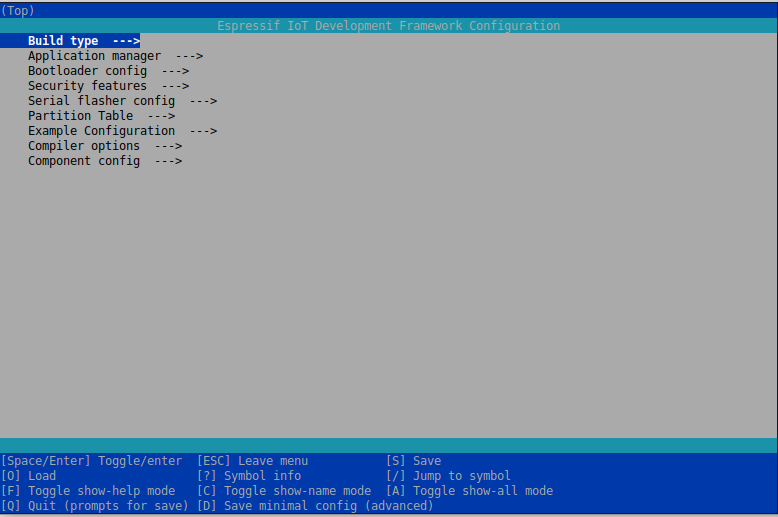
\includegraphics[width=0.7\textwidth]{images/menuConfig.png}
    \caption{Menuconfig window of the project}
    \label{fig:menuConfig} % This is the image label, with which you can refer to the image in any document location.
\end{figure}

Move through the menu using arrow keys end go in \textbf{Example Configuration} to set your personal settings (Wifi connection)
and the peer configuration of WireGuard module (or leave it as it is, to use our configuration) \ref{fig:menuConfig_ex}.

Remember:
\begin{itemize}
    \item \textbf{Wireguard Private Key}: set the private key of the client peer
    \item \textbf{Wireguard remote peer public key}: set the public key of the peer of the server
    \item \textbf{Wireguard local IP address}: set the static IP address of the client peer
    \item \textbf{Wireguard remote peer address}: set the IP address assigned by the router to the server (see NOTE in section \ref{sec:WGprog})
    \item \textbf{Wireguard local/remote peer port}: set the ports for the UDP comunication
    \item \textbf{Target IP address or name}: set the static IP address assigned to the peer server from the server configuration \ref{sec:server}
\end{itemize}

\begin{figure}[H]
    \vspace{0.4cm}
    \centering
    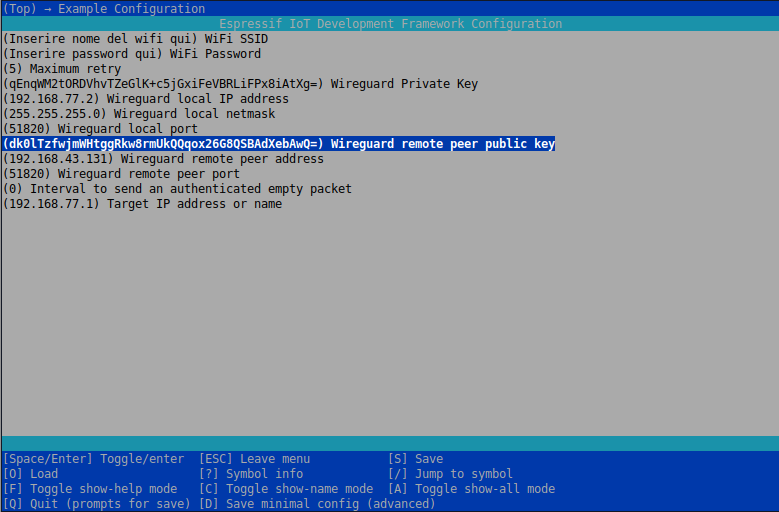
\includegraphics[width=0.7\textwidth]{images/menuConfig_ex.png}
    \caption{Example configuration window in Menuconfig}
    \label{fig:menuConfig_ex} % This is the image label, with which you can refer to the image in any document location.
\end{figure}

\subsection{Build the Project}
Remember to set the environment variable \ref{sec:envSetup} if not done.
Build the project by running:
\begin{lstlisting}
    idf.py build
\end{lstlisting}

This command will compile the application and all ESP-IDF components, then it will generate the bootloader, partition table, and application binaries. 
The first time the command is executed will be slow, then each time a small change is done the build is going to be faster.

\subsection{Connect the Device}
Now connect the ESP32 board to the computer and check under which serial port the board is visible.
\\On Linux the serial ports have \texttt{/dev/tty} naming patterns. So, in order to understand the name of the port assigned to the ESP32
run the command \texttt{ls /dev/tty*} two times, before and after connecting the device and check the difference.
Usually if there are no other USB connections the assigned port should be \texttt{/dev/ttyUSB0}.
Add the User to the dialout group using the following command:
\begin{lstlisting}
    adduser <user_name> dialout
\end{lstlisting} 

\textbf{NOTE}: In case a VM on Windows is used, remember to install the \textit{Silicon Labs CP2102 USB to UART Bridge Controller} driver
on Windows. After that, go under \textbf{Machine $\rightarrowtail$ Settings $\rightarrowtail$ USB} in the VirtualBox Menu bar and add a new USB filter (the plus icon) selecting the correct one

\begin{figure}[H]
    \vspace{0.4cm}
    \centering
    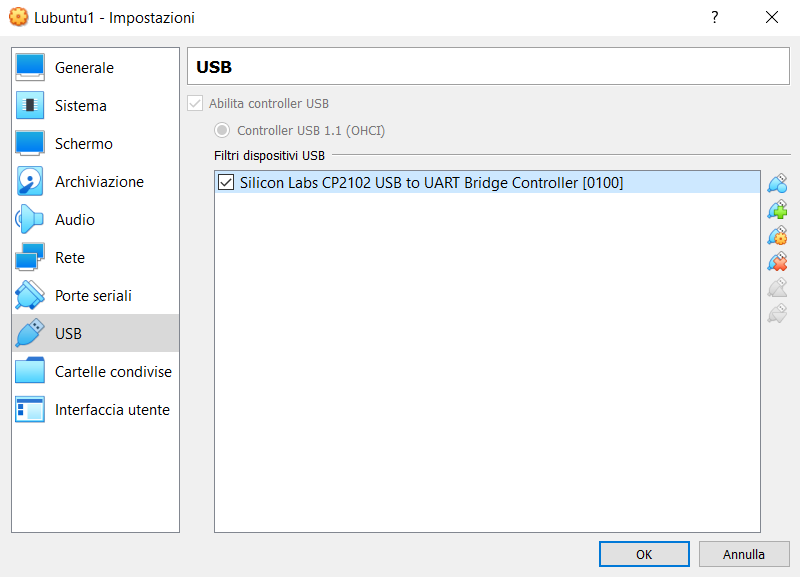
\includegraphics[width=0.75\textwidth]{images/USBex.PNG}
    \caption{Set the USB connection through Oracle VirtualBox VM.}
    \label{fig:USBex} % This is the image label, with which you can refer to the image in any document location.
\end{figure}

\subsection{Flash and Monitor the Device}
Remember to set the environment variable \ref{sec:envSetup} if not done.
Flash the binaries that were built onto the ESP32 board by running:
\begin{lstlisting}
    idf.py -p PORT [-b BAUD] flash
\end{lstlisting}

Replace PORT with the ESP32 board’s serial port name (i.e. /dev/ttyUSB0).
\\To check if the project is indeed running, type the following command that launches the IDF Monitor application:
\begin{lstlisting}
    idf.py -p PORT monitor
\end{lstlisting}

\textbf{Remember}: To exit IDF monitor use the shortcut \texttt{Ctrl+{]}}.

The two commands can be combined in one:
\begin{lstlisting}
    idf.py -p PORT flash monitor
\end{lstlisting}

\subsection{Run the project}
Turn on the Virtual Network Interface on the Server \ref{sec:server}, and listen on a port using Netcat\cite{Netcat} using the following command on the Linux machine running the Server:
\begin{lstlisting}
    nc [-v] -l -p 3333  
\end{lstlisting} 

Or Install "nc for Android" app from the PlayStore \cite{Netcat_android} and use the above command.

\textbf{NOTE}: In case Netcat is note installed on the selected Linux distribution, install with the following command:
\begin{lstlisting}
    sudo apt-get install -y netcat
\end{lstlisting}

After everything is up, turn on the ESP32 (i.e. connecting it to the PC) with the project already flashed.
Other details about the project are explained in \ref{sec:wireguard} 

\section{Start the TCP/IP WG project on FreeRTOS simulator for Linux}\label{sec:WGRtos}
This project is located in the \textbf{Posix\_GCC\_lwip2\_wg} directory.
Here are reported the steps to run the project described in section \ref{sec:addwglinuxsection} starting from the execution of a blinky to download all the needed files.

\subsection{Build a simple "blinky" example}\label{sub:linux_blink}
Follow this procedure to build a simple blinky example from the demo folder of the FreeRTOS distribution.
In order to execute a general project on FreeRTOS simulator for Linux the following steps must be followed. 
\begin{enumerate}
    \item Install some common prerequisite packages: native \textbf{gcc} (the same used to build Linux applications) and \textbf{cmake}.
    \begin{lstlisting}
        sudo apt install gcc cmake
    \end{lstlisting}
    \item Download Freertos: the version used for this project is the one reported here \cite{freertosdownload}.
    \begin{lstlisting}
    git clone https://github.com/FreeRTOS/FreeRTOS.git
    \end{lstlisting}
    \item Make a copy of sample: \texttt{FreeRTOS/Demo/Posix\_GCC}.
    
    This blinky example is made of a software timer (which executes a call-back every 2 seconds) and a thread (infinite loop with a timed wait of 200 ms). Both write a single byte into a message queue on every iteration. Another thread waits for bytes to show up in the queue, recognizes the sender and writes a message for each on \texttt{stdout}.
    \item Build without modification: \texttt{make} inside \texttt{FreeRTOS/Demo/Posix\_GCC}
    
    The project is built using a Makefile: the variable \texttt{SOURCE\_FILES} contains all the source files to be compiled, and the variable \texttt{INCLUDE\_DIRS} is the concatenation of all the include paths to be passed to the compiler command. You may also want to edit \texttt{FREERTOS\_DIR\_REL} at the top of the Makefile if you move the sample to a different folder relative to the FreeRTOS distribution.
    \item run: \texttt{./build/posix\_demo} 
    
    or what you specified in the variables \texttt{BIN} and \texttt{BUILD\_DIR} in the Makefile.
\end{enumerate}

\subsection{Set up TAP}
Set up the TAP on the device, more details here \ref{TapInfo}.
\begin{enumerate}
    \item \texttt{sudo ip tuntap add dev tap1 mode tap user `whoami`} \textit{\# the tap will be called tap1 and be property of the current user}
    \item \texttt{sudo ip link set dev tap1 up}
    \item \texttt{sudo ip addr add 192.168.2.1/24 dev tap1} \textit{\# the computer assigns this address to the interface}
    \item \texttt{export PRECONFIGURED\_TAPIF=tap1} \textit{\# Set the environment variable}
\end{enumerate}

\subsection{Build and run the TCP/IP WG project}
Copy the directory \textbf{Posix\_GCC\_lwip2\_wg} inside \texttt{FreeRTOS/Demo} directory.
In order to set up the WireGuard configuration, change the needed variables inside \texttt{main\_blinky.c} according to the settings of the Client and Server.
Open a Terminal and run Netcat\cite{Netcat} opening the 3333 port:
\begin{lstlisting}
    nc -l -v 3333
\end{lstlisting}

Open a Terminal in the project directory (remember to set up the TAP environment variable) and build:

\begin{lstlisting}
    make
\end{lstlisting}

Execute:
\begin{lstlisting}
    ./build/posix_demo
\end{lstlisting}

\section{Server Configuration}\label{sec:server}
In this section it is analysed how to configure WireGuard on the server side. It is recommended to use a Linux device or an Android device. 
The following instructions are for 3 different types of application:
\begin{itemize}
    \item Linux command line
    \item Windows application
    \item Android application
\end{itemize}

\subsection{Linux server}
In order to setup WireGuard on a Linux environment it is necessary first of all to install the software running
\begin{lstlisting}
sudo apt install wireguard
\end{lstlisting}
Then must be created a private and a public keys for the Wireguard server 
\begin{lstlisting}
wg genkey               # generate private key
echo "<private key>" | wg pubkey    # generate public key
\end{lstlisting}
or to run both commands in the same line and write the keys on two distinct files in the current directory.
\begin{lstlisting} 
wg genkey | tee private.key | wg pubkey > public.key
\end{lstlisting}
At this point remains to decide the IP addresses for the tunnel. A range of IPs could be selected for the interface (i.e. 192.168.77.1/24) that will be the potential values for the available peers.
Now all the required parameters are set and the wg0.conf file could be configured. In this file must be described the interface of the server and the peers (see in section \ref{sec:WGprog} to more details) with code similar to the following one:
\begin{lstlisting}
[Interface]
Address = 192.168.77.1/24
ListenPort = 51820  # default
PrivateKey = {private key}

[Peer]
PublicKey = {public key}
AllowedIPs = 192.168.77.2/32
\end{lstlisting}
The values of the keys are the one generated before and the IPs of the peer must remain in the range of the interface.
Go in the \texttt{/etc/wireguard} and make a new \texttt{wg0.conf} file (must be admin to access the directory).

\begin{lstlisting}
sudo -i
cd /etc/wireguard
nano wg0.conf
\end{lstlisting}

Set up UFW firewall rules to open required ports:

\begin{lstlisting}
sudo ufw allow 51820/udp
\end{lstlisting}

Verify it:

\begin{lstlisting}
sudo ufw status
\end{lstlisting}

Turn the WireGuard service at boot time using the systemctl command, run:
\begin{lstlisting}
sudo systemctl enable wg-quick@wg0
\end{lstlisting}

Start the service, execute:
\begin{lstlisting}
sudo systemctl start wg-quick@wg0
\end{lstlisting}

Get the service status, run:
\begin{lstlisting}
sudo systemctl status wg-quick@wg0
\end{lstlisting}

Verify that interface named wg0 is up and running using the ip command:
\begin{lstlisting}
sudo wg
sudo ip a show wg0
\end{lstlisting}

Done! The WireGuard Server is working.

Remember to use the following commands to turn up or down the Virtual Network Interface
\begin{lstlisting} 
wg-quick up wg0
wg-quick down wg0
\end{lstlisting}

\textbf{NOTE}: In case of using Linux on Oracle VirtualBox VM the network settings of the virtual machine must be adjusted accordingly to server settings.
Go to \textbf{Machine $\rightarrowtail$ Settings $\rightarrowtail$ Network} under Menu bar, make sure it is attached to \texttt{NAT}.
Go under \textbf{Advanced $\rightarrowtail$ Port Forwarding} then add two new forwarding rules with the plus button.
Add a rule for the TCP communication and one for the UDP. An example is shown in \ref{fig:Forwarding} 

\begin{figure}[H]
    \vspace{0.4cm}
    \centering
    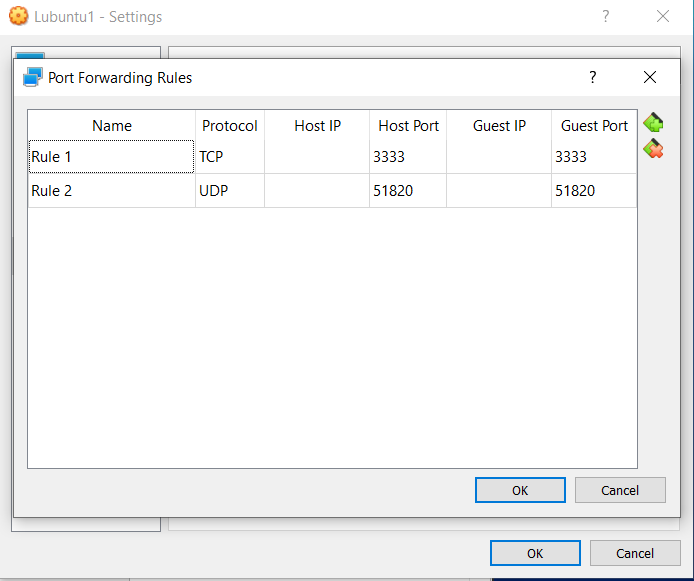
\includegraphics[width=0.75\textwidth]{images/Forwarding.PNG}
    \caption{Forwarding rules for Oracle VirtualBox VM.}
    \label{fig:Forwarding} % This is the image label, with which you can refer to the image in any document location.
\end{figure}

\subsection{Windows server}
On windows it is first of all necessary to install the WireGuard tool from the following link \cite{WireGuardDownload}.
Now you can open the GUI of the tool and create a new tunnel, using the bottom-left button (\ref{fig:wireguard_windows}), where you can create a new empty tunnel or import one from a file. in figure \ref{fig:wireguard_windows_tunnel_settings} there is an example of how to create a new empty tunnel test where there are:
\begin{itemize}
    \item one private interface, that specifies 
    \begin{itemize}
        \item a private key
        \item the listen port of the connection
        \item the address of the network interface
    \end{itemize}
    \item one peer, represented by
    \begin{itemize}
        \item a public key
        \item a range of allowed IPs (in this case only one peer is configured)
    \end{itemize}
\end{itemize}
Once the tunnel is correctly created you can activate it using the activation button, or modify the previous parameters using the bottom-right button.

\begin{figure}[H]
\vspace{0.5cm}
\centering
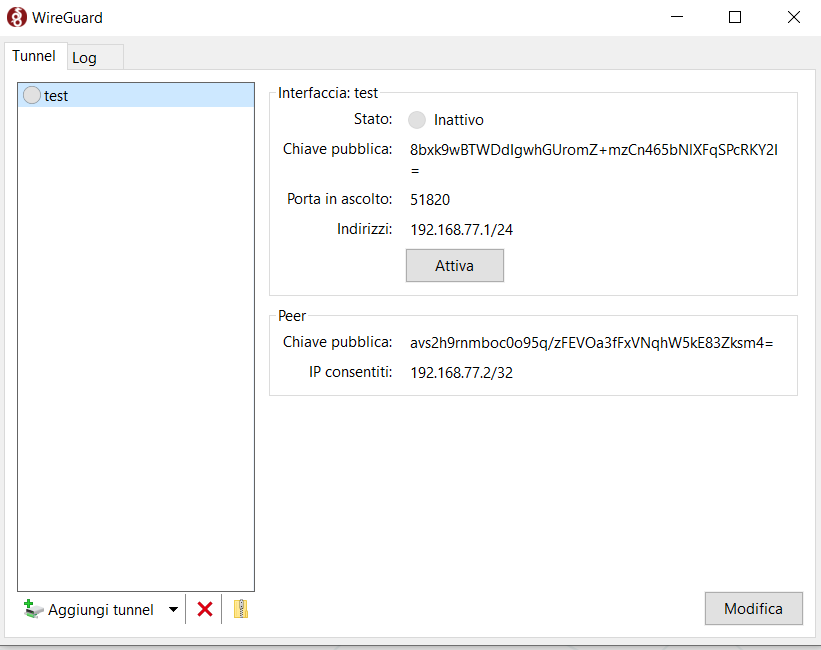
\includegraphics[width=\textwidth/3*2]{images/wireguard_windows.png}
\caption{WireGuard windows application main page.}
\label{fig:wireguard_windows} % This is the image label, with which you can refer to the image in any document location.
\end{figure}

\begin{figure}[H]
\vspace{0.5cm}
\centering
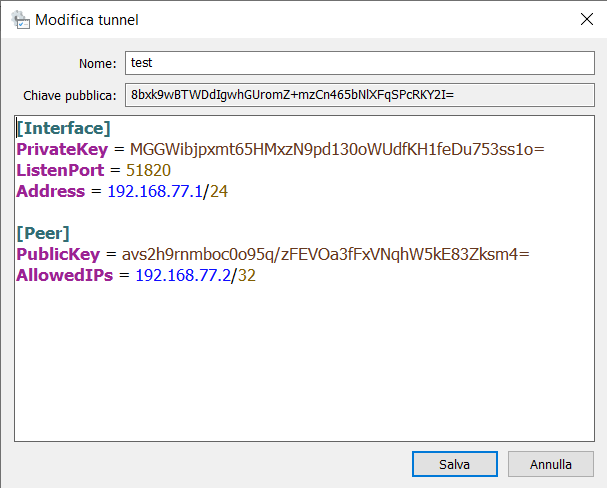
\includegraphics[width=\textwidth/3*2]{images/wireguard_windows_tunnel_settings.png}
\caption{WireGuard windows tunnel settings.}
\label{fig:wireguard_windows_tunnel_settings} % This is the image label, with which you can refer to the image in any document location.
\end{figure}

\subsection{Android server}
Also in this case the first thing to do is to download the application (from the Google Play Store). At the start-up appears the main page (left picture in \ref{fig:android_wireguard_main}), then you can click on the blue button and, selecting for example "build from scratch", you want to create a new tunnel. Now, a page with all the required settings will appear. As explained before must be set the name, the private key and the address for the network interface. Then clicking on "add peer" a peer could be added and could be set also here the public key and the range of IPs. At this point all the setting must be saved pressing the icon in the top-right corner and, using the button shown in the figure on the far right, could be turned on the corresponding tunnel.

\begin{figure}[H]
\vspace{0.5cm}
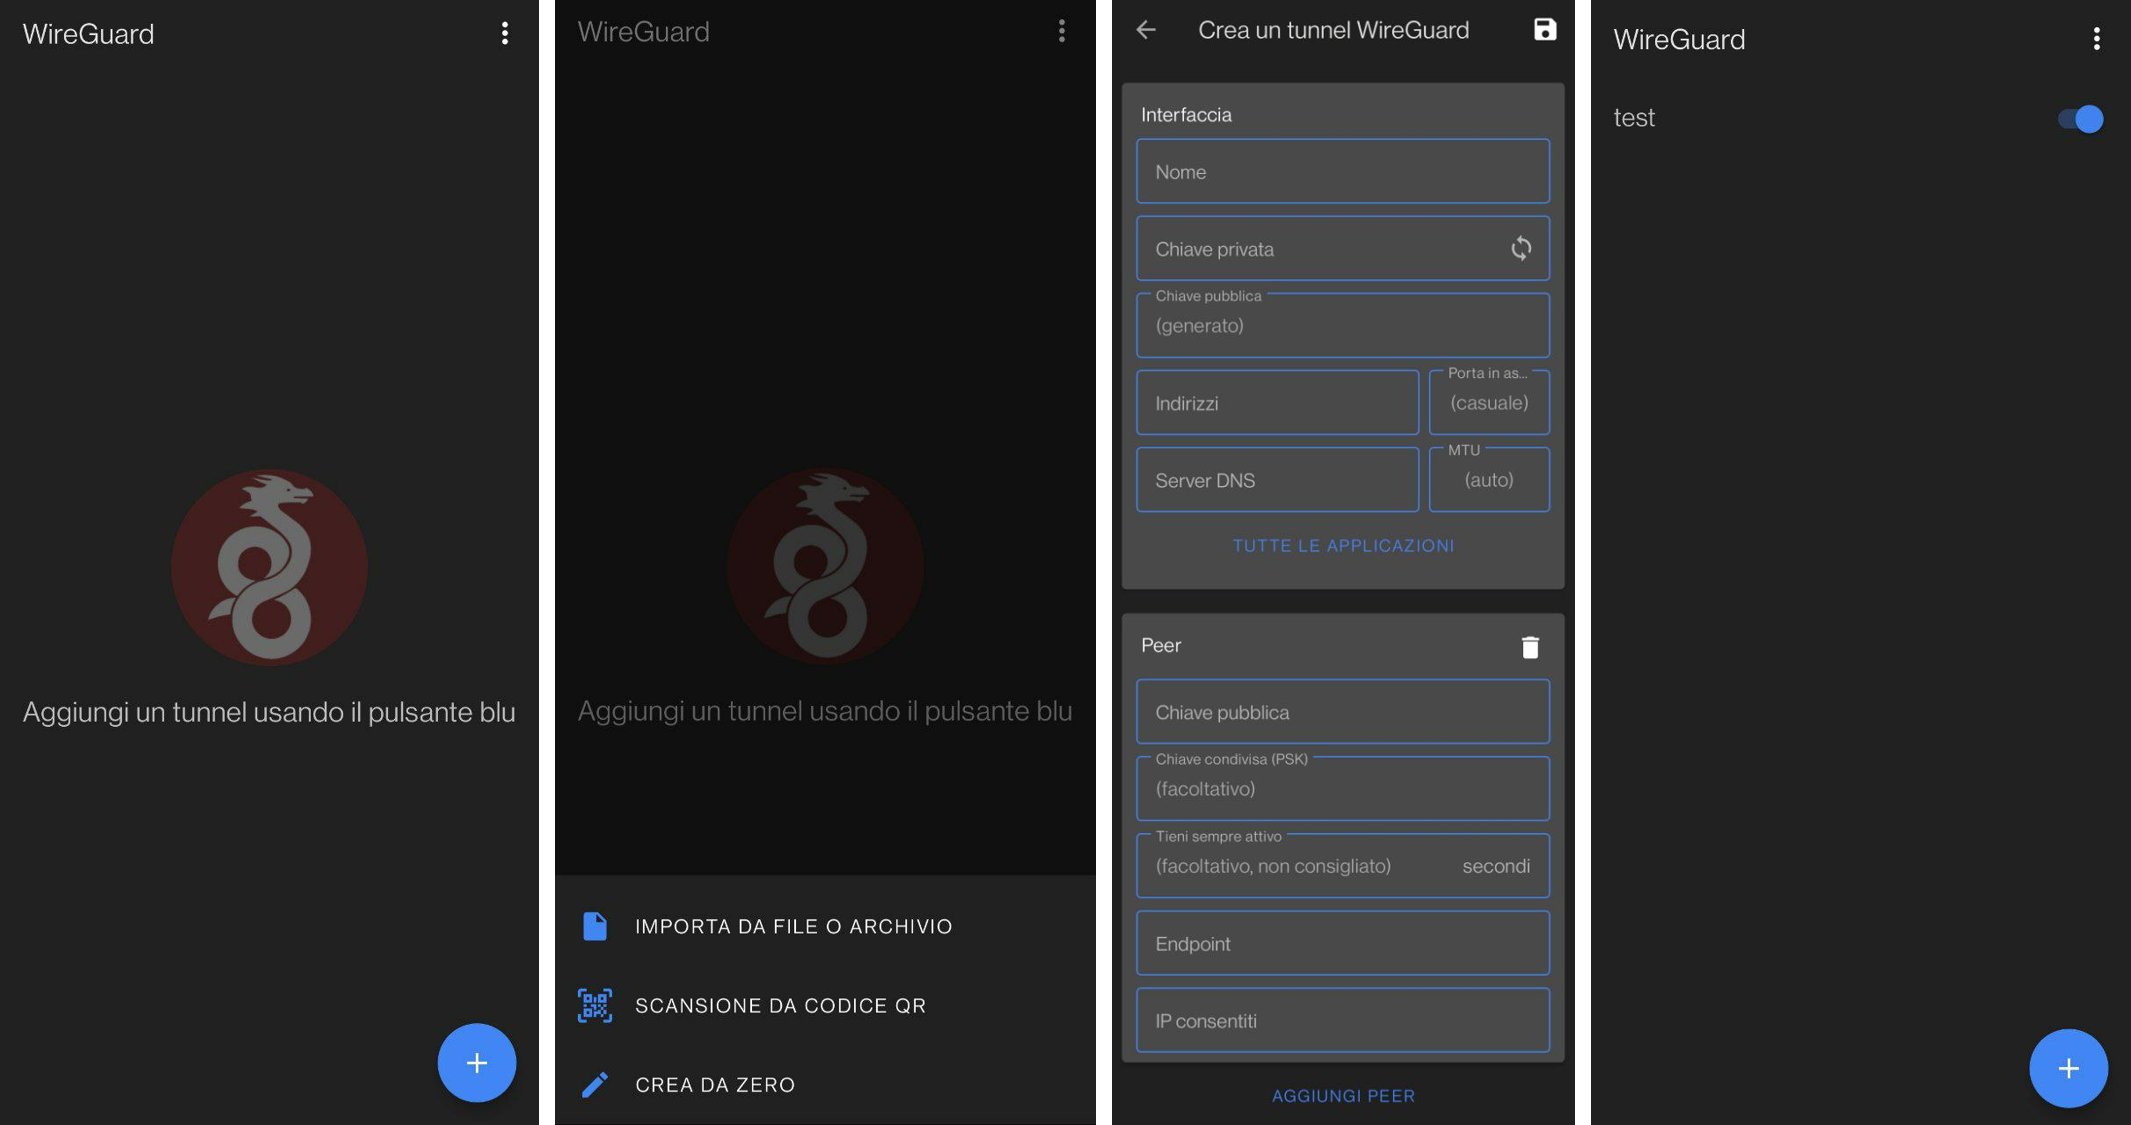
\includegraphics[width=\textwidth]{images/android_server_wg.png}
\caption{WireGuard android application.}
\label{fig:android_wireguard_main} % This is the image label, with which you can refer to the image in any document location.
\end{figure}





\printbibliography

%%%%%%%%%%%%%%%%%%%%%%%%%%%%%%%%%%%%%%%%%%%%%%%%%%%%%

\end{document}